\documentclass[a4paper,11pt,oneside,titlepage,openright]{book}
\usepackage[italian]{babel}              % italiano
%\usepackage[latin1]{inputenc}   % accenti
\usepackage[utf8]{inputenc}   % accenti
\usepackage{indentfirst}
\usepackage[dvips]{graphicx}    % per includere i grafici
\usepackage{amssymb}            % per i simboli matematici
\usepackage{amsmath}            %            "
\usepackage{latexsym}           %            "
\usepackage{amsthm}             %            "
\usepackage{amsfonts}
\usepackage{lettrine}           % per il capolettera dell'introduzione
\usepackage{epsfig}             % per includere le figure
\usepackage{hyperref}
\usepackage{graphicx}
\usepackage{color}
\usepackage{courier}
\usepackage{caption}
\usepackage{mdwlist}
\usepackage{listings}
\usepackage[T1]{fontenc}
\usepackage{booktabs}
\usepackage{longtable}
\usepackage{pdflscape}
\usepackage{rotating}
\usepackage[babel]{csquotes}
\usepackage{epigraph}
\usepackage{tabularx}
\usepackage[style=numeric-comp,useprefix,hyperref,backend=bibtex]{biblatex}
\bibliography{tex_files/bibliografia/bibliografia}


\pagestyle{headings}

\lstdefinelanguage{JavaScript}{
  keywords={typeof, new, true, false, catch, function, return, null, catch, switch, var, if, in, while, do, else, case, break},
  keywordstyle=\color{blue}\bfseries,
  ndkeywords={class, export, boolean, throw, implements, import, this},
  ndkeywordstyle=\color{darkgray}\bfseries,
  identifierstyle=\color{black},
  sensitive=false,
  comment=[l]{//},
  morecomment=[s]{/*}{*/},
  commentstyle=\color{purple}\ttfamily,
  stringstyle=\color{red}\ttfamily,
  morestring=[b]',
  morestring=[b]"
}


\DeclareCaptionFont{white}{\color{white}}
\DeclareCaptionFormat{listing}{\colorbox[cmyk]{0.43, 0.35, 0.35,0.01}{\parbox{\textwidth}{\hspace{15pt}#1#2#3}}}
\captionsetup[lstlisting]{format=listing,labelfont=white,textfont=white, singlelinecheck=false, margin=0pt, font={bf,footnotesize}}


\definecolor{lightgray}{rgb}{.9,.9,.9}
\definecolor{darkgray}{rgb}{.4,.4,.4}
\definecolor{purple}{rgb}{0.65, 0.12, 0.82}
\definecolor{Brown}{cmyk}{0,0.81,1,0.60}
\definecolor{OliveGreen}{cmyk}{0.64,0,0.95,0.40}
\definecolor{CadetBlue}{cmyk}{0.62,0.57,0.23,0}
\definecolor{lightlightgray}{gray}{0.9}





% per l'interlinea
\linespread{1.5}

\newcommand{\minisizeurl}[1]{\footnotesize #1 \normalsize}

\newcommand{\terminale}{
    \lstset{language={}}
}

\newcommand{\javascript}{
    \lstset{
    language=JavaScript,
    backgroundcolor=\color{lightgray},
    extendedchars=true,
    basicstyle=\footnotesize\ttfamily,
    showstringspaces=false,
    showspaces=false,
%    numbers=left,
%    numberstyle=\footnotesize,
%    numbersep=9pt,
    tabsize=2,
    breaklines=true,
    showtabs=false,
    captionpos=b
   }
}

\newcommand{\html}{
    \lstset{
    language=HTML,                          % Code langugage
    basicstyle=\ttfamily\footnotesize,       % Code font, Examples: \footnotesize, \ttfamily
    keywordstyle=\color{OliveGreen},        % Keywords font ('*' = uppercase)
    commentstyle=\color{gray},              % Comments font
    %numbers=left,                           % Line nums position
    %numberstyle=\tiny,                      % Line-numbers fonts
    stepnumber=1,                           % Step between two line-numbers
    numbersep=5pt,                          % How far are line-numbers from code
    backgroundcolor=\color{lightgray}, % Choose background color
    frame=none,                             % A frame around the code
    tabsize=2,                              % Default tab size
    captionpos=b,                           % Caption-position = bottom
    breaklines=true,                        % Automatic line breaking?
    breakatwhitespace=false,                % Automatic breaks only at whitespace?
    showspaces=false,                       % Dont make spaces visible
    showtabs=false,                         % Dont make tabls visible
    stringstyle=\color{red}\ttfamily,
    xleftmargin=17pt,
    framexleftmargin=17pt,
    framexrightmargin=5pt,
    framexbottommargin=4pt,
    }
}

\newcommand{\xml}{
  \lstset{
    language=XML,                          % Code langugage
    basicstyle=\ttfamily\footnotesize,       % Code font, Examples: \footnotesize, \ttfamily
    keywordstyle=\color{OliveGreen},        % Keywords font ('*' = uppercase)
    commentstyle=\color{gray},              % Comments font
    %numbers=left,                          % Line nums position
    %numberstyle=\tiny,                     % Line-numbers fonts
    stepnumber=1,                           % Step between two line-numbers
    numbersep=5pt,                          % How far are line-numbers from code
    backgroundcolor=\color{lightgray},      % Choose background color
    frame=none,                             % A frame around the code
    tabsize=2,                              % Default tab size
    captionpos=b,                           % Caption-position = bottom
    breaklines=true,                        % Automatic line breaking?
    breakatwhitespace=false,                % Automatic breaks only at whitespace?
    showspaces=false,                       % Dont make spaces visible
    showtabs=false,                         % Dont make tabls visible
    stringstyle=\color{red}\ttfamily,
    xleftmargin=17pt,
    framexleftmargin=17pt,
    framexrightmargin=5pt,
    framexbottommargin=4pt,
    }
}

%% per le estensioni
\newcommand{\ext}{png}

%% per le definizioni
\newcommand{\definizione}[1]{{\em {\bfseries #1}}}

%%VisPro maiuscoletto
\newcommand{\vp}{V{\textsc is}P{\textsc ro} }
\newcommand{\vpunspaced}{V{\textsc is}P{\textsc ro}}


%% comandi per la customizzazione della stringa dei riferimenti
\newcommand{\vedi}[1]{(si veda #1)}

\hyphenation{sil-la-ba-zio-ne}                   % per la corretta sillabazione delle parole
\hyphenation{del-le} \hyphenation{pa-ro-le}

% per gli esempi
\theoremstyle{plain}
\newtheorem{thm}{Teorema}[section]
\theoremstyle{definition}
\newtheorem{defn}{Definizione}[chapter]
\newtheorem{ex}{Esempio}[chapter]               % [CHAPTER] per la numerazione degli esempi
\theoremstyle{remark}
\newtheorem{codifica}{Codifica}

%%% DOCUMENT %%%

\begin{document}

\baselineskip=12mm
\thispagestyle{empty}

\begin{figure}
\begin{center}
~~\centerline {
\psfig{file=images/logo/logo.png,width=5cm}}
\end{center}
\end{figure}

\vskip 1.40cm

\begin{center}
\large
Università degli Studi \textit{``Roma Tre''}\\
Facoltà di Ingegneria\\
Corso di Laurea Magistrale in Ingegneria Informatica\\
\end{center}

\vskip 1cm \Large

\begin{center}
Tesi di laurea magistrale
\end{center}

\vskip 1cm \baselineskip=10mm

\begin{center}
\textbf{{\em Titolo della tesi}}\\
\end{center}

\vskip .5cm

\begin{center}
Laureando\\
{Andrea D'Amelio, Tiziano Sperati}\\
\end{center}

\vskip 1cm

\begin{center}
\large{
\begin{tabularx}{\textwidth}{>{\centering\arraybackslash}X >{\centering\arraybackslash}X}
  Relatore & Correlatori\\
  Prof. Alberto Paoluzzi & Dott.~Enrico Marino, Dott.~Federico Spini\\
\end{tabularx}
}
\end{center}

\vskip 1.5cm

\centerline{Anno Accademico 2014/2015}

\normalsize


\newpage

\newpage\null\thispagestyle{empty}\newpage
\thispagestyle{empty}
\begin{flushright}
\null\vspace{\stretch{1}}
{\em Dedicated to my family} \\
{\em and ...}
\vspace{\stretch{2}}\null
\end{flushright}

% \newpage\null\thispagestyle{empty}\newpage
\thispagestyle{empty}
\begin{flushright}
\null\vspace{\stretch{1}}
{\em To my family} \\
{\em and ...}
\vspace{\stretch{2}}\null
\end{flushright}

% \newpage\null\thispagestyle{empty}\newpage
\thispagestyle{empty}
\begin{flushright}
\null\vspace{\stretch{1}}
{\em Dedicated to my family} \\
{\em and ...}
\vspace{\stretch{2}}\null
\end{flushright}

\frontmatter

\tableofcontents

\listoffigures

\chapter{Acknowledgements}
\label{cha:acknowledgements}

Thanks to...


% \chapter{Acknowledgements}
\label{cha:acknowledgements}

Thanks to Francesco Totti


% \chapter{Acknowledgements}
\label{cha:acknowledgements}

Thanks to...


\chapter{Introduction}
\label{cha:introduction}

Since the beginning of Internet, the ability to create and publish content on the web has made the success of Content Management Systems. Products like Joomla! or WordPress, born to handle simple websites or blogs, are evolved to support web applications of any sort (from personal portfolio to online shopping), running as of January 2015 more than 25\% of the top ten million websites \cite{cms_stats}. This evolution has been allowed by a plug-in based architecture, where each plug-in is responsible to handle a functionality subset of the whole application, presenting the user through a simple accessible configuration and management interface.
The large number of available plug-ins covers most of the common and frequently required customizations, thus avoiding to write ad-hoc code. Nevertheless, the implementation of specific functional characteristics inevitably requires to intervene at code level.

When the effort required to add custom features to a CMS results too expensive, a web framework can be adopted instead. A web framework consists of a set of software facilities that aims to alleviate the overhead associate with common development activities. Web application coding effort, while eased by the web framework, is anyway rewarded with an increased level of extensibility and customizability of the resulting application.
The most desirable features for a web framework are: user management, session management, database access via HTTP RESTful API. In order to effectively speed up web applications development, these facilities should be provided relying mostly on external configuration files and less on procedural code \cite{MIPRO}.

In this thesis a software platform named X-Project is introduced. It consists of a Web Component library, a development methodology and a set of guidelines.

The Web Components library is applied over a powerful web framework, Loopback by Strongloop, and realizes an hybrid prototypal tool which brings together the customizability of a modern web framework with the ease of use of traditional CMSs.

It has been naturally prompt by the use of the toolkit and, then, standardized a document-driven development process that polarizes the concept of reusing the code whose overall readability, maintainability and extendibility result dramatically increased.

Guidelines have been drafted in order to provide an aid to users to get the straight of the entire structure.

First goal of this project is the creation of a platform that can wrap the features of CMSs and web application frameworks. 
X-Project aims to simplify developers life in web applications creation and give them the chance to easily compose, via web components libraries, pages made of reused components.
Reusability and access to reusable components is an important feature that X-Project borrows from Web Components standard.
As further said in \ref{sec:XPR_xpr}, ``Everything is an element, even a service'' is the X-Project's philosophy: every kind of function or structure is encapsulated in Polymer elements, carrying to extreme levels web components concept. 
Moreover, using Single Page Application pattern, X-Project tries to streamline loading times of web applications.

The choice of cutting edge technologies, such as Polymer-Project by Google, has been done both to meet the challenge of new and unknown development pattern, and to test the newest technologies.

X-Project is located at the end of a natural path composed by user oriented CMSs and developer oriented web application framework (see \ref{sec:CMS_class}), trying to fuse CMSs ease of use with web application frameworks customization level.

The remainder of this document is divided in two parts and organized as follows. Part One counts of three chapters. Chapter One describes the state of the art of CMS's world, giving a classification and focusing on four of the major CMSs on the market. Chapter Two analyzes every used technology, describing the methodological approach of each one. Chapter Three provides an overview of Single Page Application development pattern, explaining pros and cons and technical functioning.
Part two is composed by four chapters. Chapter Four describes the project in its integrity, exposing the core of X-Project, its functionalities and its features.
Chapter Five focuses on a specific component that has been developed, Media Management Component with S3 service, and on all the theorical and practical concepts that there's behind the ideation of the component. Chapter Six presents a real use case with configuration steps and code snippets.
Finally, Chapter Six, exposes project conclusions and further implementations of the work.





%Since the beginning of Internet, the ability to create and publish content on the web has made the success of Content Management Systems. Products like Joomla! or WordPress, born to handle simple websites or blogs, are evolved to support web applications of any sort (from personal portfolio to online shopping), running as of January 2015 more than 25\% of the top ten million websites \cite{cms_stats}. This evolution has been allowed by a plug-in based architecture, where each plug-in is responsible to handle a functionality subset of the whole application, presenting the user through a simple accessible configuration and management interface.
The large number of available plug-ins covers most of the common and frequently required customizations, thus avoiding to write ad-hoc code. Nevertheless, the implementation of specific functional characteristics inevitably requires to intervene at code level.

When the effort required to add custom features to a CMS results too expensive, a web framework can be adopted instead. A web framework consists of a set of software facilities that aims to alleviate the overhead associate with common development activities. Web application coding effort, while eased by the web framework, is anyway rewarded with an increased level of extensibility and customizability of the resulting application.
The most desirable features for a web framework are: user management, session management, database access via HTTP RESTful API. In order to effectively speed up web applications development, these facilities should be provided relying mostly on external configuration files and less on procedural code \cite{MIPRO}.

In this thesis a software platform named X-Project is introduced. It consists of a Web Component library, a development methodology and a set of guidelines.

The Web Components library is applied over a powerful web framework, Loopback by Strongloop, and realizes an hybrid prototypal tool which brings together the customizability of a modern web framework with the ease of use of traditional CMSs.

It has been naturally prompt by the use of the toolkit and, then, standardized a document-driven development process that polarizes the concept of reusing the code whose overall readability, maintainability and extendibility result dramatically increased.

Guidelines have been drafted in order to provide an aid to users to get the straight of the entire structure.

First goal of this project is the creation of a platform that can wrap the features of CMSs and web application frameworks. 
X-Project aims to simplify developers life in web applications creation and give them the chance to easily compose, via web components libraries, pages made of reused components.
Reusability and access to reusable components is an important feature that X-Project borrows from Web Components standard.
As further said in \ref{sec:XPR_xpr}, ``Everything is an element, even a service'' is the X-Project's philosophy: every kind of function or structure is encapsulated in Polymer elements, carrying to extreme levels web components concept. 
Moreover, using Single Page Application pattern, X-Project tries to streamline loading times of web applications.

The choice of cutting edge technologies, such as Polymer-Project by Google, has been done both to meet the challenge of new and unknown development pattern, and to test the newest technologies.

X-Project is located at the end of a natural path composed by user oriented CMSs and developer oriented web application framework (see \ref{sec:CMS_class}), trying to fuse CMSs ease of use with web application frameworks customization level.

The remainder of this document is divided in two parts and organized as follows. Part One counts of three chapters. Chapter One describes the state of the art of CMS's world, giving a classification and focusing on four of the major CMSs on the market. Chapter Two analyzes every used technology, describing the methodological approach of each one. Chapter Three provides an overview of Single Page Application development pattern, explaining pros and cons and technical functioning.
Part two is composed by four chapters. Chapter Four describes the project in his integrity, exposing the core of X-Project, its functionalities and its features.
Chapter Five focuses on a specific component that has been developed, User Management Component, and on all the theorical and practical things that there's behind the ideation of the component. Chapter Six presents a real use case with configuration steps and code snippets.
Finally, Chapter Six, exposes project conclusions and further implementations of the work.





Sin da le origini di Internet, la possibilità di creare e pubblicare contenuti sul web ha fatto sì che i Content Management Systems prendessero piede e avessero successo. Prodotti come Joomla! o WordPress, nati per gestire siti web o semplici blog, si sono evoluti per supportare applicazioni web di qualsiasi tipo (dal portfolio personale allo shopping on-line). Da statistiche di gennaio 2015 risulta che oltre il 25 \% dei primi dieci milioni di siti web è gestito con i maggiori CMS\cite{cms_stats}. Questa evoluzione è stata permessa da un architettura basata su plug-in, dove ogni plug-in è responsabile di gestire un sottoinsieme di funzionalità di tutta l'applicazione, presentandoso all'utente attraverso una semplice interfaccia di configurazione e una gestione estremamente accessibile.
Il gran numero di plug-in disponibile copre la maggior parte delle personalizzazioni più comunemente richieste, evitando così la scrittura di codice ad-hoc. Tuttavia, l'attuazione di specifiche caratteristiche funzionali richiede inevitabilmente l'intervento dello sviluppatore a livello di codice.

%Since the beginning of Internet, the ability to create and publish content on the web has made the success of Content Management Systems. Products like Joomla! or WordPress, born to handle simple websites or blogs, are evolved to support web applications of any sort (from personal portfolio to online shopping), running as of January 2015 more than 25\% of the top ten million websites \cite{cms_stats}. This evolution has been allowed by a plug-in based architecture, where each plug-in is responsible to handle a functionality subset of the whole application, presenting the user through a simple accessible configuration and management interface.
The large number of available plug-ins covers most of the common and frequently required customizations, thus avoiding to write ad-hoc code. Nevertheless, the implementation of specific functional characteristics inevitably requires to intervene at code level.

When the effort required to add custom features to a CMS results too expensive, a web framework can be adopted instead. A web framework consists of a set of software facilities that aims to alleviate the overhead associate with common development activities. Web application coding effort, while eased by the web framework, is anyway rewarded with an increased level of extensibility and customizability of the resulting application.
The most desirable features for a web framework are: user management, session management, database access via HTTP RESTful API. In order to effectively speed up web applications development, these facilities should be provided relying mostly on external configuration files and less on procedural code \cite{MIPRO}.

In this thesis a software platform named X-Project is introduced. It consists of a Web Component library, a development methodology and a set of guidelines.

The Web Components library is applied over a powerful web framework, Loopback by Strongloop, and realizes an hybrid prototypal tool which brings together the customizability of a modern web framework with the ease of use of traditional CMSs.

It has been naturally prompt by the use of the toolkit and, then, standardized a document-driven development process that polarizes the concept of reusing the code whose overall readability, maintainability and extendibility result dramatically increased.

Guidelines have been drafted in order to provide an aid to users to get the straight of the entire structure.

First goal of this project is the creation of a platform that can wrap the features of CMSs and web application frameworks. 
X-Project aims to simplify developers life in web applications creation and give them the chance to easily compose, via web components libraries, pages made of reused components.
Reusability and access to reusable components is an important feature that X-Project borrows from Web Components standard.
As further said in (\ref{sec:XPR_xpr}), ``Everything is an element, even a service'' is the X-Project's philosophy: every kind of function or structure is encapsulated in Polymer elements, carrying to extreme levels web components concept. 
Moreover, using Single Page Application pattern, X-Project tries to streamline loading times of web applications.

The choice of cutting edge technologies, such as Polymer-Project by Google, has been done both to meet the challenge of new and unknown development pattern, and to test the newest technologies.

X-Project is located at the end of a natural path composed by user oriented CMSs and developer oriented web application framework (see \ref{sec:CMS_class}), trying to fuse CMSs ease of use with web application frameworks customization level.

The remainder of this document is divided in two parts and organized as follows. Part One counts of three chapters. Chapter One describes the state of the art of CMS's world, giving a classification and focusing on four of the major CMSs on the market. Chapter Two analyzes every used technology, describing the methodological approach of each one. Chapter Three provides an overview of Single Page Application development pattern, explaining pros and cons and technical functioning.
Part two is composed by four chapters. Chapter Four describes the project in his integrity, exposing the core of X-Project, its functionalities and its features.
Chapter Five focuses on a specific component that has been developed, User Management Component, and on all the theorical and practical things that there's behind the ideation of the component. Chapter Six presents a real use case with configuration steps and code snippets.
Finally, Chapter Six, exposes project conclusions and further implementations of the work.







\chapter{Introduzione}
\label{cha:introduzione}

\section{Introduzione(ITA)}

Sin da le origini di Internet, la possibilità di creare e pubblicare contenuti sul web ha fatto sì che i Content Management Systems prendessero piede e avessero successo. Prodotti come Joomla! o WordPress, nati per gestire siti web o semplici blog, si sono evoluti per supportare applicazioni web di qualsiasi tipo (dal portfolio personale allo shopping on-line). Da statistiche di gennaio 2015 risulta che oltre il 25 \% dei primi dieci milioni di siti web è gestito con i maggiori CMS\cite{cms_stats}. Questa evoluzione è stata permessa da un architettura basata su plug-in, dove ogni plug-in è responsabile di gestire un sottoinsieme di funzionalità di tutta l'applicazione, presentandosi all'utente attraverso una semplice interfaccia di configurazione e una gestione estremamente accessibile.
Il gran numero di plug-in disponibile copre la maggior parte delle personalizzazioni più comunemente richieste, evitando così la scrittura di codice ad-hoc. Tuttavia, l'attuazione di specifiche caratteristiche funzionali richiede inevitabilmente l'intervento dello sviluppatore a livello di codice.

Quando lo sforzo richiesto per aggiungere funzioni personalizzate a un CMS risulta troppo costoso, è utile adottare un web framework. Un web framework è costituito da una serie di servizi software che mira ad alleviare il lavoro con comuni attività di sviluppo. Lo sforzo di codifica delle Applicazioni Web, sebbene venga facilitato dal web framework, è comunque premiato con una maggiore possibilità di estensione e personalizzazione dell'applicazione risultante.
Le caratteristiche più desiderabili per un web framework sono: la gestione degli utenti, gestione delle sessioni, l'accesso al database tramite HTTP API RESTful. Al fine di velocizzare in modo efficace lo sviluppo di applicazioni web, queste strutture dovrebbero essere fornite basandosi principalmente sul file di configurazione esterni e meno sul codice di procedura \cite{MIPRO}.

In questa tesi viene introdotta una piattaforma software chiamata X-Project. Essa consiste in una una metodologia di sviluppo contornata da una libreria di componenti Web e una serie di linee guida.

La libreria dei componenti Web viene applicata su un web framework potente, Loopback di Strongloop, realizzando uno strumento prototipale ibrido che riunisce la personalizzazione di un framework web moderno con la facilità d'uso dei tradizionali CMS.

Tale libreria è nata in maniera naturale durante l'utilizzo del toolkit e, successivamente, è stato standardizzato un processo di sviluppo documento driven che polarizza il concetto di riuso del codice la cui leggibilità, manutenibilità e estendibilità risulta estremamente aumentata.

Le linee guida sono state redatte in modo da fornire un aiuto agli utenti per avere diritti su tutta la struttura

Primo obiettivo di questo progetto è la creazione di una piattaforma in grado di avvolgere le caratteristiche del CMS e di un web framework per applicazioni.
X-Project mira a semplificare la vita agli sviluppatori di applicazioni web nella creazione e dare loro la possibilità di comporre facilmente, tramite le librerie di componenti web, pagine fatte di componenti riutilizzati.
Riusabilità e l'accesso ai componenti riutilizzabili è una caratteristica importante che X-Project prende in prestito dallo standard dei Web Components.
Come detto in \ref{sec: XPR_xpr}, ``Tutto è un elemento, anche un servizio'' questa è la filosofia di X-Project: ogni tipo di funzione o di struttura è incapsulato in elementi Polymer, portando a livelli estremi il concetto dei componenti web.
Inoltre, utilizzando il modello Single Page Application, X-Project cerca di ottimizzare i tempi di caricamento delle web application.

La scelta di tecnologie all'avanguardia, come Polymer-Project di Google, è stata dettata sia dalla sfida insita nell'uso di pattern di sviluppo sconosciuti, sia dal fascino rappresentato dal ``nuovo''. 

X-Project si colloca alla fine del percorso naturale composto dai CMS orientati all'utente e dai web application framework orientati allo sviluppatore (vedi \ref{sec:CMS_class}), provando a fondere la semplicità d'utilizzo dei CMS con il livello di possibilità di personalizzazione dei web application frameworks.

Questa tesi è suddivisa in due parti ed è organizzata come segue. La Parte Uno è composta da tre capitoli. Il Capitolo Uno descrive lo stato dell'arte del mondo dei CMS, fornendo anche una classificazione per tipo e soffermandosi ad analizzare quattro dei maggiori prodotti presenti sul mercato. Il secondo capitolo analizza le tecnologie utilizzate, descrivendo l'approccio tecnico e metodologico di ognuna di esse. Il terzo capitolo fornisce una panoramica sul pattern di sviluppo detto Single Page Application, esponendone vantaggi e svantaggi ed il funzionamento tecnico.

La seconda Parte è composta da quattro capitoli. Il capitolo quattro descrive il progetto nella sua totalità, esponendo l'anima di X-Project, le funzionalità e le caratteristiche.
Il quinto e il sesto capitolo si concentrano su componenti specifici, rispettivamente, il Media Management S3 Component e lo User Management Component, e su tutti i concetti teorici e pratici che si celano dietro all'elemento finale.
Il settimo capitolo mostra un caso d'uso evidenziando, con snippet e screenshot, i punti salienti dell'implementazione di una web application tramite X-Project.
Infine, l'ottavo ed ultimo capitolo, espone le conclusioni tratte e fornisce dei possibili sviluppi futuri per il progetto.

%\section{Introduzione(ITA)}

Sin da le origini di Internet, la possibilità di creare e pubblicare contenuti sul web ha fatto sì che i Content Management Systems prendessero piede e avessero successo. Prodotti come Joomla! o WordPress, nati per gestire siti web o semplici blog, si sono evoluti per supportare applicazioni web di qualsiasi tipo (dal portfolio personale allo shopping on-line). Da statistiche di gennaio 2015 risulta che oltre il 25 \% dei primi dieci milioni di siti web è gestito con i maggiori CMS\cite{cms_stats}. Questa evoluzione è stata permessa da un architettura basata su plug-in, dove ogni plug-in è responsabile di gestire un sottoinsieme di funzionalità di tutta l'applicazione, presentandosi all'utente attraverso una semplice interfaccia di configurazione e una gestione estremamente accessibile.
Il gran numero di plug-in disponibile copre la maggior parte delle personalizzazioni più comunemente richieste, evitando così la scrittura di codice ad-hoc. Tuttavia, l'attuazione di specifiche caratteristiche funzionali richiede inevitabilmente l'intervento dello sviluppatore a livello di codice.

Quando lo sforzo richiesto per aggiungere funzioni personalizzate a un CMS risulta troppo costoso, è utile adottare un web framework. Un web framework è costituito da una serie di servizi software che mira ad alleviare il lavoro con comuni attività di sviluppo. Lo sforzo di codifica delle Applicazioni Web, sebbene venga facilitato dal web framework, è comunque premiato con una maggiore possibilità di estensione e personalizzazione dell'applicazione risultante.
Le caratteristiche più desiderabili per un web framework sono: la gestione degli utenti, gestione delle sessioni, l'accesso al database tramite HTTP API RESTful. Al fine di velocizzare in modo efficace lo sviluppo di applicazioni web, queste strutture dovrebbero essere fornite basandosi principalmente sul file di configurazione esterni e meno sul codice di procedura \cite{MIPRO}.

In questa tesi viene introdotta una piattaforma software chiamata X-Project. Essa consiste in una una metodologia di sviluppo contornata da una libreria di componenti Web e una serie di linee guida.

La libreria dei componenti Web viene applicata su un web framework potente, Loopback di Strongloop, realizzando uno strumento prototipale ibrido che riunisce la personalizzazione di un framework web moderno con la facilità d'uso dei tradizionali CMS.

Tale libreria è nata in maniera naturale durante l'utilizzo del toolkit e, successivamente, è stato standardizzato un processo di sviluppo documento driven che polarizza il concetto di riuso del codice la cui leggibilità, manutenibilità e estendibilità risulta estremamente aumentata.

Le linee guida sono state redatte in modo da fornire un aiuto agli utenti per avere diritti su tutta la struttura

Primo obiettivo di questo progetto è la creazione di una piattaforma in grado di avvolgere le caratteristiche del CMS e di un web framework per applicazioni.
X-Project mira a semplificare la vita agli sviluppatori di applicazioni web nella creazione e dare loro la possibilità di comporre facilmente, tramite le librerie di componenti web, pagine fatte di componenti riutilizzati.
Riusabilità e l'accesso ai componenti riutilizzabili è una caratteristica importante che X-Project prende in prestito dallo standard dei Web Components.
Come detto in \ref{sec: XPR_xpr}, ``Tutto è un elemento, anche un servizio'' questa è la filosofia di X-Project: ogni tipo di funzione o di struttura è incapsulato in elementi Polymer, portando a livelli estremi il concetto dei componenti web.
Inoltre, utilizzando il modello Single Page Application, X-Project cerca di ottimizzare i tempi di caricamento delle web application.

La scelta di tecnologie all'avanguardia, come Polymer-Project di Google, è stata dettata sia dalla sfida insita nell'uso di pattern di sviluppo sconosciuti, sia dal fascino rappresentato dal ``nuovo''. 

X-Project si colloca alla fine del percorso naturale composto dai CMS orientati all'utente e dai web application framework orientati allo sviluppatore (vedi \ref{sec:CMS_class}), provando a fondere la semplicità d'utilizzo dei CMS con il livello di possibilità di personalizzazione dei web application frameworks.

Questa tesi è suddivisa in due parti ed è organizzata come segue. La Parte Uno è composta da tre capitoli. Il Capitolo Uno descrive lo stato dell'arte del mondo dei CMS, fornendo anche una classificazione per tipo e soffermandosi ad analizzare quattro dei maggiori prodotti presenti sul mercato. Il secondo capitolo analizza le tecnologie utilizzate, descrivendo l'approccio tecnico e metodologico di ognuna di esse. Il terzo capitolo fornisce una panoramica sul pattern di sviluppo detto Single Page Application, esponendone vantaggi e svantaggi ed il funzionamento tecnico.

La seconda Parte è composta da quattro capitoli. Il capitolo quattro descrive il progetto nella sua totalità, esponendo l'anima di X-Project, le funzionalità e le caratteristiche.
Il quinto e il sesto capitolo si concentrano su componenti specifici, rispettivamente, il Media Management S3 Component e lo User Management Component, e su tutti i concetti teorici e pratici che si celano dietro all'elemento finale.
Il settimo capitolo mostra un caso d'uso evidenziando, con snippet e screenshot, i punti salienti dell'implementazione di una web application tramite X-Project.
Infine, l'ottavo ed ultimo capitolo, espone le conclusioni tratte e fornisce dei possibili sviluppi futuri per il progetto.

%\section{Introduzione(ITA)}

Sin da le origini di Internet, la possibilità di creare e pubblicare contenuti sul web ha fatto sì che i Content Management Systems prendessero piede e avessero successo. Prodotti come Joomla! o WordPress, nati per gestire siti web o semplici blog, si sono evoluti per supportare applicazioni web di qualsiasi tipo (dal portfolio personale allo shopping on-line). Da statistiche di gennaio 2015 risulta che oltre il 25 \% dei primi dieci milioni di siti web è gestito con i maggiori CMS\cite{cms_stats}. Questa evoluzione è stata permessa da un architettura basata su plug-in, dove ogni plug-in è responsabile di gestire un sottoinsieme di funzionalità di tutta l'applicazione, presentandosi all'utente attraverso una semplice interfaccia di configurazione e una gestione estremamente accessibile.
Il gran numero di plug-in disponibile copre la maggior parte delle personalizzazioni più comunemente richieste, evitando così la scrittura di codice ad-hoc. Tuttavia, l'attuazione di specifiche caratteristiche funzionali richiede inevitabilmente l'intervento dello sviluppatore a livello di codice.

Quando lo sforzo richiesto per aggiungere funzioni personalizzate a un CMS risulta troppo costoso, è utile adottare un web framework. Un web framework è costituito da una serie di servizi software che mira ad alleviare il lavoro con comuni attività di sviluppo. Lo sforzo di codifica delle Applicazioni Web, sebbene venga facilitato dal web framework, è comunque premiato con una maggiore possibilità di estensione e personalizzazione dell'applicazione risultante.
Le caratteristiche più desiderabili per un web framework sono: la gestione degli utenti, gestione delle sessioni, l'accesso al database tramite HTTP API RESTful. Al fine di velocizzare in modo efficace lo sviluppo di applicazioni web, queste strutture dovrebbero essere fornite basandosi principalmente sul file di configurazione esterni e meno sul codice di procedura \cite{MIPRO}.

In questa tesi viene introdotta una piattaforma software chiamata X-Project. Essa consiste in una una metodologia di sviluppo contornata da una libreria di componenti Web e una serie di linee guida.

La libreria dei componenti Web viene applicata su un web framework potente, Loopback di Strongloop, realizzando uno strumento prototipale ibrido che riunisce la personalizzazione di un framework web moderno con la facilità d'uso dei tradizionali CMS.

Tale libreria è nata in maniera naturale durante l'utilizzo del toolkit e, successivamente, è stato standardizzato un processo di sviluppo documento driven che polarizza il concetto di riuso del codice la cui leggibilità, manutenibilità e estendibilità risulta estremamente aumentata.

Le linee guida sono state redatte in modo da fornire un aiuto agli utenti per avere diritti su tutta la struttura

Primo obiettivo di questo progetto è la creazione di una piattaforma in grado di avvolgere le caratteristiche del CMS e di un web framework per applicazioni.
X-Project mira a semplificare la vita agli sviluppatori di applicazioni web nella creazione e dare loro la possibilità di comporre facilmente, tramite le librerie di componenti web, pagine fatte di componenti riutilizzati.
Riusabilità e l'accesso ai componenti riutilizzabili è una caratteristica importante che X-Project prende in prestito dallo standard dei Web Components.
Come detto in \ref{sec: XPR_xpr}, ``Tutto è un elemento, anche un servizio'' questa è la filosofia di X-Project: ogni tipo di funzione o di struttura è incapsulato in elementi Polymer, portando a livelli estremi il concetto dei componenti web.
Inoltre, utilizzando il modello Single Page Application, X-Project cerca di ottimizzare i tempi di caricamento delle web application.

La scelta di tecnologie all'avanguardia, come Polymer-Project di Google, è stata dettata sia dalla sfida insita nell'uso di pattern di sviluppo sconosciuti, sia dal fascino rappresentato dal ``nuovo''. 

X-Project si colloca alla fine del percorso naturale composto dai CMS orientati all'utente e dai web application framework orientati allo sviluppatore (vedi \ref{sec:CMS_class}), provando a fondere la semplicità d'utilizzo dei CMS con il livello di possibilità di personalizzazione dei web application frameworks.

Questa tesi è suddivisa in due parti ed è organizzata come segue. La Parte Uno è composta da tre capitoli. Il Capitolo Uno descrive lo stato dell'arte del mondo dei CMS, fornendo anche una classificazione per tipo e soffermandosi ad analizzare quattro dei maggiori prodotti presenti sul mercato. Il secondo capitolo analizza le tecnologie utilizzate, descrivendo l'approccio tecnico e metodologico di ognuna di esse. Il terzo capitolo fornisce una panoramica sul pattern di sviluppo detto Single Page Application, esponendone vantaggi e svantaggi ed il funzionamento tecnico.

La seconda Parte è composta da quattro capitoli. Il capitolo quattro descrive il progetto nella sua totalità, esponendo l'anima di X-Project, le funzionalità e le caratteristiche.
Il quinto e il sesto capitolo si concentrano su componenti specifici, rispettivamente, il Media Management S3 Component e lo User Management Component, e su tutti i concetti teorici e pratici che si celano dietro all'elemento finale.
Il settimo capitolo mostra un caso d'uso evidenziando, con snippet e screenshot, i punti salienti dell'implementazione di una web application tramite X-Project.
Infine, l'ottavo ed ultimo capitolo, espone le conclusioni tratte e fornisce dei possibili sviluppi futuri per il progetto.



% \chapter{Introduction}
\label{cha:introduction}

Since the beginning of Internet, the ability to create and publish content on the web has made the success of Content Management Systems. Products like Joomla! or WordPress, born to handle simple websites or blogs, are evolved to support web applications of any sort (from personal portfolio to online shopping), running as of January 2015 more than 25\% of the top ten million websites \cite{cms_stats}. This evolution has been allowed by a plug-in based architecture, where each plug-in is responsible to handle a functionality subset of the whole application, presenting the user through a simple accessible configuration and management interface.
The large number of available plug-ins covers most of the common and frequently required customizations, thus avoiding to write ad-hoc code. Nevertheless, the implementation of specific functional characteristics inevitably requires to intervene at code level.

When the effort required to add custom features to a CMS results too expensive, a web framework can be adopted instead. A web framework consists of a set of software facilities that aims to alleviate the overhead associate with common development activities. Web application coding effort, while eased by the web framework, is anyway rewarded with an increased level of extensibility and customizability of the resulting application.
The most desirable features for a web framework are: user management, session management, database access via HTTP RESTful API. In order to effectively speed up web applications development, these facilities should be provided relying mostly on external configuration files and less on procedural code \cite{MIPRO}.

In this thesis a software platform named X-Project is introduced. It consists of a Web Component library, a development methodology and a set of guidelines.

The Web Components library is applied over a powerful web framework, Loopback by Strongloop, and realizes an hybrid prototypal tool which brings together the customizability of a modern web framework with the ease of use of traditional CMSs.

It has been naturally prompt by the use of the toolkit and, then, standardized a document-driven development process that polarizes the concept of reusing the code whose overall readability, maintainability and extendibility result dramatically increased.

Guidelines have been drafted in order to provide an aid to users to get the straight of the entire structure.

First goal of this project is the creation of a platform that can wrap the features of CMSs and web application frameworks. 
X-Project aims to simplify developers life in web applications creation and give them the chance to easily compose, via web components libraries, pages made of reused components.
Reusability and access to reusable components is an important feature that X-Project borrows from Web Components standard.
As further said in \ref{sec:XPR_xpr}, ``Everything is an element, even a service'' is the X-Project's philosophy: every kind of function or structure is encapsulated in Polymer elements, carrying to extreme levels web components concept. 
Moreover, using Single Page Application pattern, X-Project tries to streamline loading times of web applications.

The choice of cutting edge technologies, such as Polymer-Project by Google, has been done both to meet the challenge of new and unknown development pattern, and to test the newest technologies.

X-Project is located at the end of a natural path composed by user oriented CMSs and developer oriented web application framework (see \ref{sec:CMS_class}), trying to fuse CMSs ease of use with web application frameworks customization level.

The remainder of this document is divided in two parts and organized as follows. Part One counts of three chapters. Chapter One describes the state of the art of CMS's world, giving a classification and focusing on four of the major CMSs on the market. Chapter Two analyzes every used technology, describing the methodological approach of each one. Chapter Three provides an overview of Single Page Application development pattern, explaining pros and cons and technical functioning.

Part two is composed by four chapters. Chapter Four describes the project in its entirety, exposing the core of X-Project, its functionalities and its features.
Chapter Five and six focus on specific components that have been developed, Media Management S3 Component and User Management Component, and on all the theorical and practical concepts that are behind the ideation of the component. 
Chapter seven presents a real use case highlighting, with configuration steps and code snippets the major aspects of a web application implementation with X-Project.
Finally, Chapter eight, exposes project conclusions and further implementations of the work.





Section 1

Section 2

In conclusions...



% \chapter{Introduction}
\label{cha:introduction}

Since the beginning of Internet, the ability to create and publish content on the web has made the success of Content Management Systems. Products like Joomla! or WordPress, born to handle simple websites or blogs, are evolved to support web applications of any sort (from personal portfolio to online shopping), running as of January 2015 more than 25\% of the top ten million websites \cite{cms_stats}. This evolution has been allowed by a plug-in based architecture, where each plug-in is responsible to handle a functionality subset of the whole application, presenting the user through a simple accessible configuration and management interface.
The large number of available plug-ins covers most of the common and frequently required customizations, thus avoiding to write ad-hoc code. Nevertheless, the implementation of specific functional characteristics inevitably requires to intervene at code level.

When the effort required to add custom features to a CMS results too expensive, a web framework can be adopted instead. A web framework consists of a set of software facilities that aims to alleviate the overhead associate with common development activities. Web application coding effort, while eased by the web framework, is anyway rewarded with an increased level of extensibility and customizability of the resulting application.
The most desirable features for a web framework are: user management, session management, database access via HTTP RESTful API. In order to effectively speed up web applications development, these facilities should be provided relying mostly on external configuration files and less on procedural code \cite{MIPRO}.

In this thesis a software platform named X-Project is introduced. It consists of a Web Component library, a development methodology and a set of guidelines.

The Web Components library is applied over a powerful web framework, Loopback by Strongloop, and realizes an hybrid prototypal tool which brings together the customizability of a modern web framework with the ease of use of traditional CMSs.

It has been naturally prompt by the use of the toolkit and, then, standardized a document-driven development process that polarizes the concept of reusing the code whose overall readability, maintainability and extendibility result dramatically increased.

Guidelines have been drafted in order to provide an aid to users to get the straight of the entire structure.

First goal of this project is the creation of a platform that can wrap the features of CMSs and web application frameworks. 
X-Project aims to simplify developers life in web applications creation and give them the chance to easily compose, via web components libraries, pages made of reused components.
Reusability and access to reusable components is an important feature that X-Project borrows from Web Components standard.
As further said in \ref{sec:XPR_xpr}, ``Everything is an element, even a service'' is the X-Project's philosophy: every kind of function or structure is encapsulated in Polymer elements, carrying to extreme levels web components concept. 
Moreover, using Single Page Application pattern, X-Project tries to streamline loading times of web applications.

The choice of cutting edge technologies, such as Polymer-Project by Google, has been done both to meet the challenge of new and unknown development pattern, and to test the newest technologies.

X-Project is located at the end of a natural path composed by user oriented CMSs and developer oriented web application framework (see \ref{sec:CMS_class}), trying to fuse CMSs ease of use with web application frameworks customization level.

The remainder of this document is divided in two parts and organized as follows. Part One counts of three chapters. Chapter One describes the state of the art of CMS's world, giving a classification and focusing on four of the major CMSs on the market. Chapter Two analyzes every used technology, describing the methodological approach of each one. Chapter Three provides an overview of Single Page Application development pattern, explaining pros and cons and technical functioning.

Part two is composed by four chapters. Chapter Four describes the project in its entirety, exposing the core of X-Project, its functionalities and its features.
Chapter Five and six focus on specific components that have been developed, Media Management S3 Component and User Management Component, and on all the theorical and practical concepts that are behind the ideation of the component. 
Chapter seven presents a real use case highlighting, with configuration steps and code snippets the major aspects of a web application implementation with X-Project.
Finally, Chapter eight, exposes project conclusions and further implementations of the work.





Section 1

Section 2

In conclusions...



\mainmatter

\part{Part 1}
\label{part:part_1}


\chapter{Content Management System}
\label{cha:chapter_CMS}

In this chapter...

\section{CMS Overview}
\label{sec:CMS_overview}

In this section there will be an overview about Content Management Systems.

A Content Management System is an application, that provides capabilities for multiple users with different permission levels to manage content, data or information of a website project, or internet application. [ http://www.aiim.org/What-is-Web-CMS-WCM-System-Content-Management ].

Managing content refers to creating, editing, archiving, publishing, collaborating on, reporting, distributing website content, data and information.
So, a CMS is an application that allows creating and publishing content from a central interface. CMSs are often used to run websites containing blogs, news, and shopping. Many corporate and marketing websites use CMSs. CMSs typically aim to avoid the need for hand coding, but may help it for specific elements or entire pages [https://en.wikipedia.org/wiki/Content_management_system]. 

A Web CMS may catalog and index content, select or assemble content at runtime, or deliver content to specific visitors in a requested way, such as other languages. Web Content Management System's usually allow client control over HyperText Markup Language - based content, files, documents, and Web hosting plans based on the system depth and the niche it serves.

Nel mondo dei CMS entrano in gioco 3 figure principali: lo sviluppatore, l’amministratore e l’utente. Ogni figura svolge un ruolo fondamentale per la vita di un sito web gestito tramite CMS.
Lo sviluppatore è colui che, materialmente, crea il sito web, gestisce le funzionalità e la grafica e effettua il set up per l’amministratore.
L’amministratore è una figura non tecnica (non un programmatore) che gestisce i contenuti del sito: crea, modifica, pubblica e gestisce il materiale da presentare. Egli gestisce i contenuti del sito attraverso un pannello di amministrazione creato ad hoc dallo sviluppatore, all’interno di un’area riservata.
Infine, l’utente è colui che fruisce dei contenuti immessi nel sito dall’amministratore. Non può accedere al pannello di amministrazione e, quindi, non può inserire, modificare o cancellare i contenuti (a volte è possibile commentare i contenuti esistenti).

I CMS più famosi (e.g. Joomla! e Wordpress) hanno quasi del tutto eliminato la figura dello sviluppatore, inserendo dei tool di creazione grafica e fornendo dei preset che coprono larga parte delle richieste più comuni. Altri CMS che si stanno affermando in questo momento hanno invece fatto dello sviluppatore un punto di forza, puntando molto sulla possibilità di personalizzazione e customizzazione del prodotto.8

Since the beginning of Internet, the ability to create and publish content on the web has made the success of Content Management Systems. Products like Joomla! or WordPress, born to handle simple websites or blogs, are evolved to support web applications of any sort (from personal portfolio to on-line shopping), running as of January 2015 more than 25 percent of the top ten million websites ["Usage Statistics and Market Share of Content Management Systems for Websites". W3Techs. Retrieved January 2015 - http://w3techs.com/technologies/overview/content_management/all]. This evolution has been allowed by a plug-in based architecture, where each plug-in is responsible to handle a functionality subset of the whole application, presenting the user through a simple accessible configuration and management interface.
The large number of available plug-ins covers most of the common and frequently required customizations, thus avoiding to write ad-hoc code. Nevertheless, the implementation of specific functional characteristics inevitably requires to intervene at code level.

\section{Joomla!}
\label{sec:CMS_joomla}

Joomla is a free and open-source content management system (CMS) for publishing web content. It is built on a model–view–controller web application framework that can be used independently of the CMS. NOTA 1

Joomla is written in PHP, uses object-oriented programming (OOP) techniques (since version 1.5  NOTA 2) and software design patterns, stores data in a MySQL, MS SQL (since version 2.5), or PostgreSQL (since version 3.0) database NOTA 3, and includes features such as page caching, RSS feeds, printable versions of pages, news flashes, blogs, search, and support for language internationalization.
As of February 2014, Joomla has been downloaded over 50 million times NOTA 4. Over 7,700 free and commercial extensions are available from the official Joomla! Extension Directory, and more are available from other sources. It is estimated to be the second most used content management system on the Internet, after WordPress NOTA 5. 
Like many other web applications, Joomla may be run on a LAMP stack.
Many web hosts have control panels for automatic installation of Joomla. On Windows, Joomla can be installed using the Microsoft Web Platform Installer, which automatically detects and installs dependencies, such as PHP or MySQL.
Many web sites provide information on installing and maintaining Joomla sites.

\subsection{History}
\label{joomla_his}
Joomla was the result of a fork of Mambo on August 17, 2005. At that time, the Mambo name was a trademark of Miro International Pty Ltd, who formed a non-profit foundation with the stated purpose of funding the project and protecting it from lawsuits. The Joomla development team claimed that many of the provisions of the foundation structure violated previous agreements made by the elected Mambo Steering Committee, lacked the necessary consultation with key stakeholders and included provisions that violated core open source values.
Joomla developers created a website called OpenSourceMatters.org (OSM) to distribute information to the software community. Project leader Andrew Eddie wrote a letter that appeared on the announcements section of the public forum at mamboserver.com. Over one thousand people joined OpenSourceMatters.org within a day, most posting words of encouragement and support. The website received the Slashdot effect as a result. Miro CEO Peter Lamont responded publicly to the development team in an article titled The Mambo Open Source Controversy, 20 Questions With Miro. This event created controversy within the free software community about the definition of open source. Forums of other open-source projects were active with postings about the actions of both sides.
In the two weeks following Eddie's announcement, teams were re-organized and the community continued to grow. Eben Moglen and the Software Freedom Law Center (SFLC) assisted the Joomla core team beginning in August 2005, as indicated by Moglen's blog entry from that date and a related OSM announcement. The SFLC continue to provide legal guidance to the Joomla project.
On August 18, Andrew Eddie called for community input to suggest a name for the project. The core team reserved the right for the final naming decision, and chose a name not suggested by the community. On September 22, the new name, Joomla!, was announced. It is the anglicised spelling of the Swahili word jumla meaning all together or as a whole which also has a similar meaning in at least Amharic, Arabic and Urdu. On September 26, the development team called for logo submissions from the community and invited the community to vote on the logo; the team announced the community's decision on September 29. On October 2, brand guidelines, a brand manual, and a set of logo resources were published.
Joomla won the Packt Publishing Open Source Content Management System Award in 2006, 2007, and 2011 NOTA 6. 


\subsection{Extensions}
\label{subsec:joomla_ext}
Joomla extensions extend the functionality of Joomla websites. Five types of extensions may be distinguished: components, modules, plugins, templates, and languages. Each of these extensions handles a specific function.
\begin{itemize}
	\item Components are the largest and most complex extensions. Most components have two parts: a site part and an administrator part. Every time a Joomla page loads, one component is called to render the main page body. Components produce the major portion of a page because a component is driven by a menu item.
	\item Plugins are advanced extensions and are, in essence, event handlers. In the execution of any part of Joomla, a module or a component, an event may be triggered. When an event is triggered, plugins that are registered to handle that event execute. For example, a plugin could be used to block user-submitted articles and filter text. The line between plugins and components can sometimes be a little fuzzy. Sometimes large or advanced plugins are called components even though they don't actually render large portions of a page. An SEF URL extension might be created as a component, even though its functionality could be accomplished with just a plugin.
	\item Templates describe the main design of a Joomla website. While the CMS manages the website content, templates determine the style or look and feel and layout of a site.
	\item Modules render pages in Joomla. They are linked to Joomla components to display new content or images. Joomla modules look like boxes, such as the search or login module. However, they don’t require html in Joomla to work.
	\item Languages are very simple extensions that can either be used as a core part or as an extension. Language and font information can also be used for PDF or PSD to Joomla conversions NOTA 6. 
\end{itemize}




\begin {figure}[h]
\graphicspath{{images/chapter_cms/}}
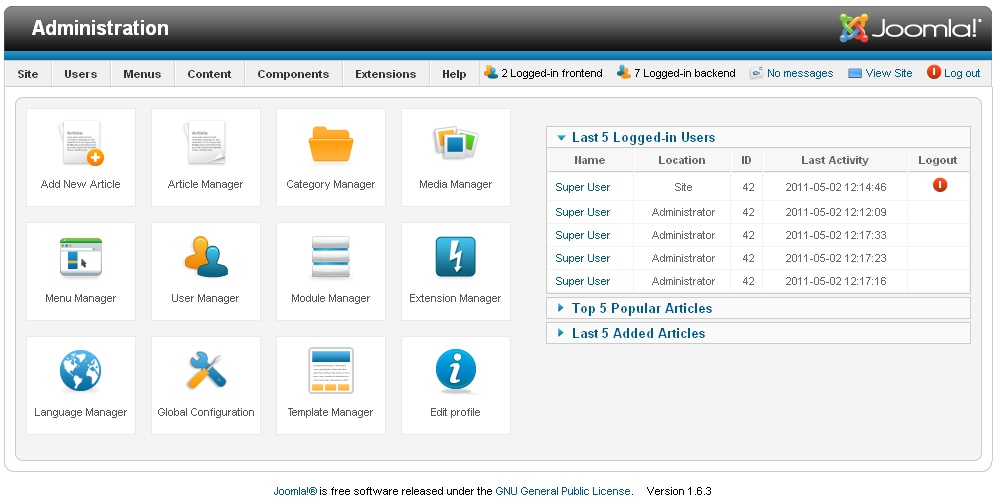
\includegraphics[width=\textwidth]{joomla_dash}
\caption{Joomla! Dashboard}
\end {figure}


\section{Wordpress}
\label{sec:CMS_wp}

WordPress is a free and open-source content management system (CMS) based on PHP and MySQL. \cite{cms_wp_over} Features include a plugin architecture and a template system. WordPress was used by more than 23.3\%of the top 10 million websites as of January 2015. WordPress is the most popular blogging system in use on the Web, at more than 60 million websites \cite{cms_wp_stats}.


\subsection{History}
\label{subsec:wp_his}
It was first released on May 27, 2003, by its founders, Matt Mullenweg and Mike Little, as a fork of b2/cafelog. The license under which WordPress software is released is the GPLv2 (or later) from the Free Software Foundation.
b2/cafelog, more commonly known as simply b2 or cafelog, was the precursor to WordPress. b2/cafelog was estimated to have been installed on approximately 2,000 blogs as of May 2003. It was written in PHP for use with MySQL by Michel Valdrighi, who is now a contributing developer to WordPress. Although WordPress is the official successor, another project, b2evolution, is also in active development.
WordPress first appeared in 2003 as a joint effort between Matt Mullenweg and Mike Little to create a fork of b2. Christine Selleck Tremoulet, a friend of Mullenweg, suggested the name WordPress.
In 2004 the licensing terms for the competing Movable Type package were changed by Six Apart, resulting in many of its most influential users migrating to WordPress. By October 2009 the Open Source CMS MarketShare Report concluded that WordPress enjoyed the greatest brand strength of any open-source content-management system \cite{cms_wp}. 



\subsection{Themes}
\label{subsec:wp_themes}


WordPress has a web template system using a template processor.
WordPress users may install and switch between themes. Themes allow users to change the look and functionality of a WordPress website and they can be installed without altering the content or health of the site. Every WordPress website requires at least one theme to be present and every theme should be designed using WordPress standards with structured PHP, valid HTML and CSS. Themes may be directly installed using the WordPress Appearance administration tool in the dashboard or theme folders may be uploaded via FTP. The PHP, HTML (HyperText Markup Language) and CSS (Cascading Style Sheets) code found in themes can be added to or edited for providing advanced features. WordPress themes are in general classified into two categories, free themes and premium themes. All the free themes are listed in the WordPress theme directory and premium themes should be purchased from marketplaces and individual WordPress developers. WordPress users may also create and develop their own custom themes if they have the knowledge and skill to do so. If WordPress users do not have themes development knowledge then they may download and use free WordPress themes from wordpress.org \cite{cms_wp}. 

\subsection{Plugins}
\label{subsec:wp_plugins}


WordPress's plugin architecture allows users to extend the features and functionality of a website or blog. WordPress has over 39,078 plugins available, each of which offers custom functions and features enabling users to tailor their sites to their specific needs. These customizations range from search engine optimization, to client portals used to display private information to logged in users, to content displaying features, such as the addition of widgets and navigation bars. But not all available plugins are always abreast with the upgrades and as a result they may not function properly or may not function at all \cite{cms_wp}.



\begin {figure}[h]
\graphicspath{{images/chapter_cms/}}
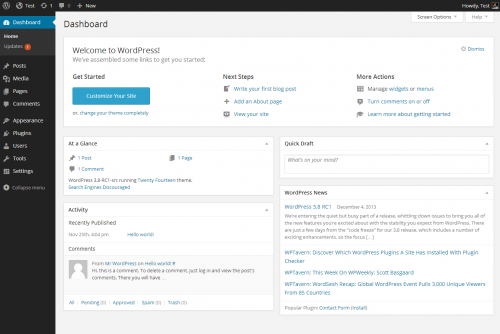
\includegraphics[width=\textwidth]{wp_dash}
\caption{WordPress Dashboard}
\end {figure}


\paragraph{}
This chapter describes the word of CMSs and provides the analysis and a classification of this environment. Finally, it describes thefour main CMSs currently on the marcket that fit two categories previously identified.



\chapter{Tecnologie Abilitanti e Scelte di Progetto}
\label{cha:chapter_TCH}

In this chapter...

\section{HTML 5}
\label{sec:TCH_html5}

In this section there will be an overview about Html5.

HTML5 is the latest version of Hypertext Markup Language, the code that describes web pages. It's actually three kinds of code: HTML, which provides the structure; Cascading Style Sheets (CSS), which take care of presentation; and JavaScript, which makes things happen.

HTML5 has been designed to deliver almost everything you'd want to do online without requiring additional software such as browser plugins. It does everything from animation to apps, music to movies, and can also be used to build incredibly complicated applications that run in your browser.

There's more. HTML5 isn't proprietary, so you don't need to pay royalties to use it. It's also cross-platform, which means it doesn't care whether you're using a tablet or a smartphone, a netbook, notebook or ultrabook or a Smart TV: if your browser supports HTML5, it should work flawlessly. Inevitably, it's a bit more complicated than that. More about that in a moment.

While some features of HTML5 are often compared to Adobe Flash, the two technologies are very different. Both include features for playing audio and video within web pages, and for using Scalable Vector Graphics. HTML5 on its own cannot be used for animation or interactivity – it must be supplemented with CSS3 or JavaScript. There are many Flash capabilities that have no direct counterpart in HTML5. See Comparison of HTML5 and Flash.

Although HTML5 has been well known among web developers for years, its interactive capabilities became a topic of mainstream media around April 2010 after Apple Inc's then-CEO Steve Jobs issued a public letter titled Thoughts on Flash where he concluded that ``Flash is no longer necessary to watch video or consume any kind of web content'' and that ``new open standards created in the mobile era, such as HTML5, will win''.This sparked a debate in web development circles where some suggested that while HTML5 provides enhanced functionality, developers must consider the varying browser support of the different parts of the standard as well as other functionality differences between HTML5 and Flash. In early November 2011, Adobe announced that it would discontinue development of Flash for mobile devices and reorient its efforts in developing tools using HTML5.


\section{Web Components}
\label{sec:TCH_webcomponents}

This section provides an overview of Web Components.

Web Components are a set of standards currently being produced by Google engineers as a W3C specification that allows for the creation of reusable widgets or components in web documents and web applications. The intention behind them is to bring component-based software engineering to the World Wide Web. The components model allows for encapsulation and interoperability of individual HTML elements.

Support for Web Components is present in some WebKit-based browsers like Google Chrome and Opera and is in Mozilla Firefox (requires a manual configuration change). Microsoft's Internet Explorer has not implemented any Web Components specifications yet.[1] Backwards compatibility with older browsers is implemented using JavaScript-based polyfills.\cite{tch_webcomp}

\begin {figure}[h]
\graphicspath{{images/chapter_TCH/}}
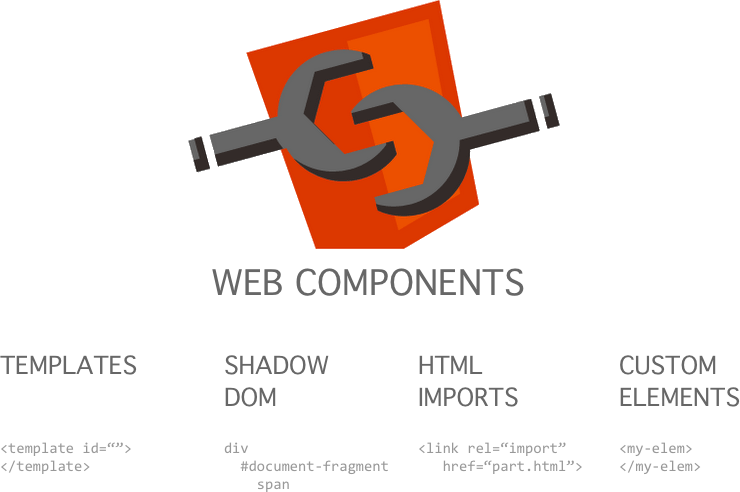
\includegraphics[width=\textwidth]{webcomponents_1}
\end {figure}

Web Components consist of 4 main elements which can be used separately or all together:

\begin{itemize}

\item Custom Elements 

Custom Elements allow authors to define their own custom HTML elements. Authors associate JavaScript code with custom tag names, and then use those custom tag names as they would any standard tag. Custom elements are still elements. It is possible to create, use, manipulate, and compose them just as easily as any standard <div> or <span> today.\cite{tch_custom}

\item Shadow DOM

Shadow DOM addresses the lack of true DOM tree encapsulation when building components. With Shadow DOM, elements can get a new kind of node associated with them. This new kind of node is called a shadow root. An element that has a ``shadow root'' associated with it is called a ``shadow host''. The content of a shadow host isn’t rendered; the content of the shadow root is rendered instead. Shadow DOM allows a single node to express three subtrees: light DOM, shadow DOM, and composed DOM. Together, the light DOM and shadow DOM are referred to as the logical DOM. This is the DOM that the developer interacts with. The composed DOM is what the browser sees and uses to render the pixels on the screen.\cite{tch_dom}

\emph{Structure of a Shadow DOM}
An element that has a shadow root associated with it is called shadow host. The shadow root can be treated as an ordinary DOM element, so it is possible to append arbitrary nodes to it. With Shadow DOM, all markup and CSS are scoped to the host element. In other words, CSS styles defined inside a Shadow Root won't affect its parent document, CSS styles defined outside the Shadow Root won't affect the main page.

\item HTML Import 

This webcomponents.js repository contains a JavaScript polyfill for the HTML Imports specification.
HTML Imports are a way to include and reuse HTML documents in other HTML documents. As <script> tags let authors include external JavaScript in their pages, imports let authors load full HTML resources. In particular, imports let authors include Custom Element definitions from external URLs.

\item Templates

This specification describes a method for declaring inert DOM subtrees in HTML and manipulating them to instantiate document fragments with identical contents.
\end{itemize}



\section{Polymer}
\label{sec:TCH_polymer}

In this section there will be an overview about Polymer.

The specifications introduced above are quite new and it is hardly surprising to know that browser support is not very good. But, thanks to the Polymer library, created by the awesome folks at Google, we can use all these features in modern browsers today. Polymer provides a set of polyfills that enables us to use web components in non-compliant browsers with an easy-to-use framework. Polymer does this by:

Allowing us to create Custom Elements with user-defined naming schemes. These custom elements can then be distributed across the network and used by others with HTML Imports.

Allowing each custom element to have its own template accompanied by styles and behavior required to use that element.

Providing a suite of ready-made UI and non-UI elements to use and extend in your project.

The elements collection of Polymer is divided into more sections:

\begin{itemize}

\item Core Elements — These are a set of visual and non-visual elements designed to work with the layout, user interaction, selection, and scaffolding applications.
\item Paper Elements — Implements the material design philosophy launched by Google recently at Google I/O 2014, and these include everything from a simple button to a dialog box with neat visual effects.
\item Iron Elements — A set of visual and non-visual utility elements. Includes elements for working with layout, user input, selection, and scaffolding apps.
\item Gold Elements — The gold elements are built for e-commerce use-cases like checkout flows.
\item Neon Elements — Neon elements implement special effects.
\item Platinum Elements — Elements to turn your web page into a true webapp, with push, offline, and more.
\item Molecules — Molecules are elements that wrap other javascript libraries.
\end{itemize}
HTML provides a set of built-in elements like <button>, <form> and <table>. Each element has its own API of attributes, properties, methods, and events. Each element has built-in styling, as well as style properties you can override using CSS.

Anyone can use these elements to build a simple web page. But they’re limited. To build something as simple as a set of tabs, you need HTML plus CSS and usually a script, too.

Web components. These standards provide the primitives you need to build new components. You can build your own custom elements using these primitives, but it can be a lot of work.
The Polymer library. Provides a declarative syntax that makes it simpler to define custom elements. And it adds features like templating, two-way data binding and property observation to help you build powerful, reusable elements with less code.
Custom elements. If you don’t want to write your own elements, there are a number of elements built with Polymer that you can drop straight into your existing pages. These elements depend on the Polymer library, but you can use the elements without using Polymer directly.

Polymer is one of the first implementations of a user interface library built upon the Web Components standard.  Web Components are not fully supported by browsers, but they provide a polyfill library, webcomponents.js, that provides enough functionality to support Web Components and Polymer.
Web Components is the result of the evolution of user interface libraries over the past decade.  At one point, we strove to separate our HTML, CSS, and JavaScript and ran our HTML through W3C validators. This led to unintended complexities…  For example, looking at a .css file, you couldn’t easily determine which selectors are actually used in your HTML and especially programmatically used in JavaScript.  Similarly, your JavaScript code was difficult to organize so that code could be reused efficiently on multiple pages.


\section{NodeJS}
\label{sec:TCH_nodejs}

In this section there will be an overview about NodeJs.

Node.js is an open source, cross-platform runtime environment for server-side and networking applications. Node.js applications are written in JavaScript and can be run within the Node.js runtime on OS X, Microsoft Windows, Linux, FreeBSD, NonStop,IBM AIX, IBM System z and IBM i. Its work is hosted and supported by the Node.js Foundation,a Collaborative Project at Linux Foundation.

Node.js provides an event-driven architecture and a non-blocking I/O API that optimizes an application's throughput and scalability. These technologies are commonly used for real-time web applications.

Node.js uses the Google V8 JavaScript engine to execute code, and a large percentage of the basic modules are written in JavaScript. Node.js contains a built-in library to allow applications to act as a Web server without software such as Apache HTTP Server, Nginx or IIS.

Node.js allows the creation of web servers and networking tools, using JavaScript and a collection of "modules" that handle various core functionality. Modules handle file system I/O, networking (HTTP, TCP, UDP, DNS, or TLS/SSL), binary data (buffers), cryptography functions, data streams , and other core functions. Node's modules have a simple and elegant API, reducing the complexity of writing server applications.

Frameworks can be used to accelerate the development of applications, and common frameworks are Express.js, Socket.IO and Connect. Node.js applications can run on Microsoft Windows, Unix, NonStop and Mac OS X servers. Node.js applications can alternatively be written with CoffeeScript (an alternative form of JavaScript), Dart or Microsoft TypeScript (strongly typed forms of JavaScript), or any language that can compile to JavaScript.

Node.js is primarily used to build network programs such as web servers, making it similar to PHP and Python. The biggest difference between PHP and Node.js is that PHP is a blocking language (commands execute only after the previous command has completed), while Node.js is a non-blocking language (commands execute in parallel, and use callbacks to signal completion).

Node.js brings event-driven programming to web servers, enabling development of fast web servers in JavaScript. Developers can create highly scalable servers without using threading, by using a simplified model of event-driven programming that uses callbacks to signal the completion of a task. Node.js was created because concurrency is difficult in many server-side programming languages, and often leads to poor performance. Node.js connects the ease of a scripting language (JavaScript) with the power of Unix network programming.


\section{MongoDB}
\label{sec:TCH_mongodb}

This section provides an overview of MongoDB.

MongoDB is a cross-platform document-oriented database. Classified as a NoSQL database, 
MongoDB eschews the traditional table-based relational database structure in favor of JSON-like documents with dynamic schemas (MongoDB calls the format BSON), making the integration of data in certain types of applications easier and faster. Released under a combination of the GNU Affero General Public License and the Apache License, MongoDB is free and open-source software.

MongoDB was created by Dwight Merriman and Eliot Horowitz, who had encountered development and scalability issues with traditional relational database approaches while building Web applications at DoubleClick, an Internet advertising company that is now owned by Google Inc. According to Merriman, the name of the database was derived from the word humongous to represent the idea of supporting large amounts of data. Merriman and Horowitz helped form 10Gen Inc. in 2007 to commercialize MongoDB and related software. The company was renamed MongoDB Inc. in 2013. 

The database was released to open source in 2009 and is available under the terms of the Free Software Foundation's GNU AGPL Version 3.0 commercial license. At the time of this writing, among other users, the insurance company MetLife is using MongoDB for customer service applications, the website Craigslist is using it for archiving data, the CERN physics lab is using it for data aggregation and discovery and the The New York Times newspaper is using MongoDB to support a form-building application for photo submissions.


\begin {figure}[h]
\graphicspath{{images/chapter_TCH/}}
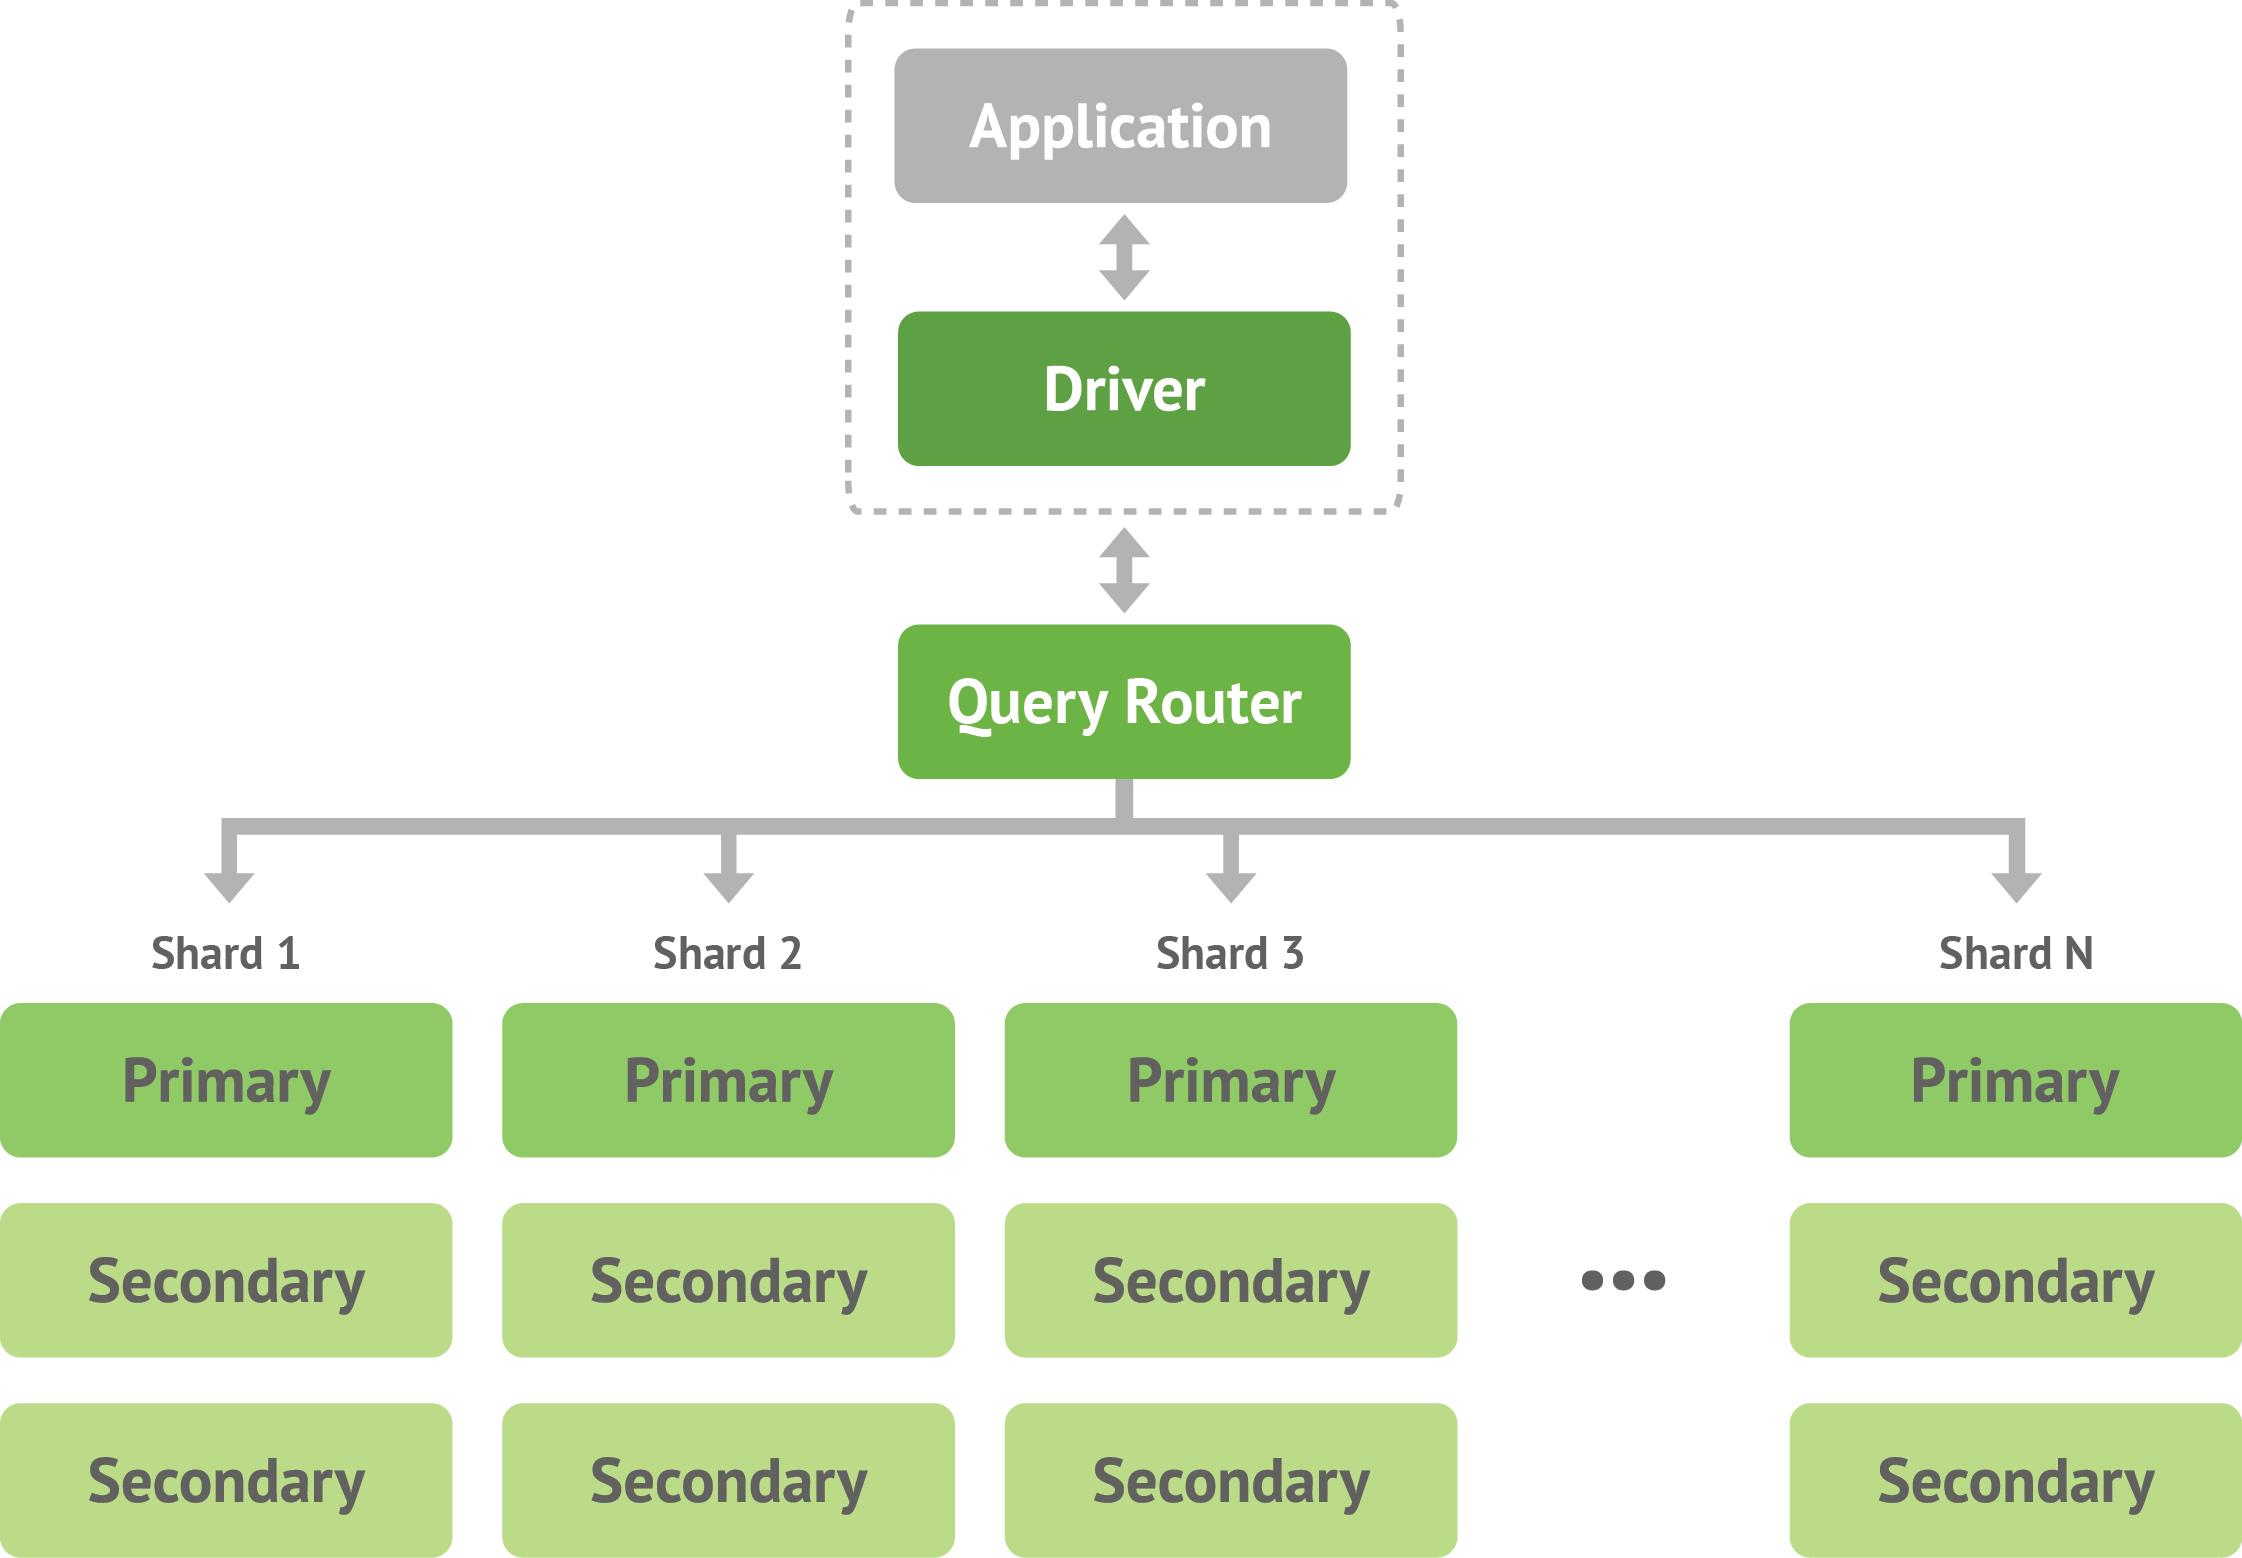
\includegraphics[width=\textwidth]{mongodb_1}
\caption{MongoDB Architecture}
\end {figure}

\section{StrongLoop LoopBack}
\label{sec:TCH_loopback}

In this section there will be an overview about LoopBack.

Built on top of the open source LoopBack framework, the StrongLoop API Platform is the first end-to-end platform for the full API lifecycle that allows you to visually develop REST APIs in Node and get them connected to new and legacy data. In addition, the API Platform features built-in mBaaS features like push and offline sync, plus graphical tools with DevOps features for clustering, profiling and monitoring Node apps.

LoopBack generates model API from the models schemas, to let CRUD operations on models.

LoopBack models automaticaly have a standard set of HTTP endpoints that provide REST APIs for create, read, update, and delete (CRUD) operations on model data:
\begin{itemize}
\item POST /Model — Create a new instance of the model and persist it into the data source.
\item GET /Model — Find all instances of the model matched by filter from the data source.
\item PUT /Model — Update an existing model instance or insert a new one into the data source.
\item PUT /Model/{id} — Update attributes for a model instance and persist it into the data source.
\item GET /Model/{id} — Find a model instance by id from the data source.
\item DELETE /Model/{id} — Delete a model instance by id from the data source.
\item GET /Model/count — Count instances of the model matched by where from the data source.
\item GET /Model/findOne Find first instance of the model matched by filter from the data source.
\item POST /Model/update — Update instances of the model matched by where from that data source.
\end{itemize}


\begin {figure}[h]
\graphicspath{{images/chapter_TCH/}}
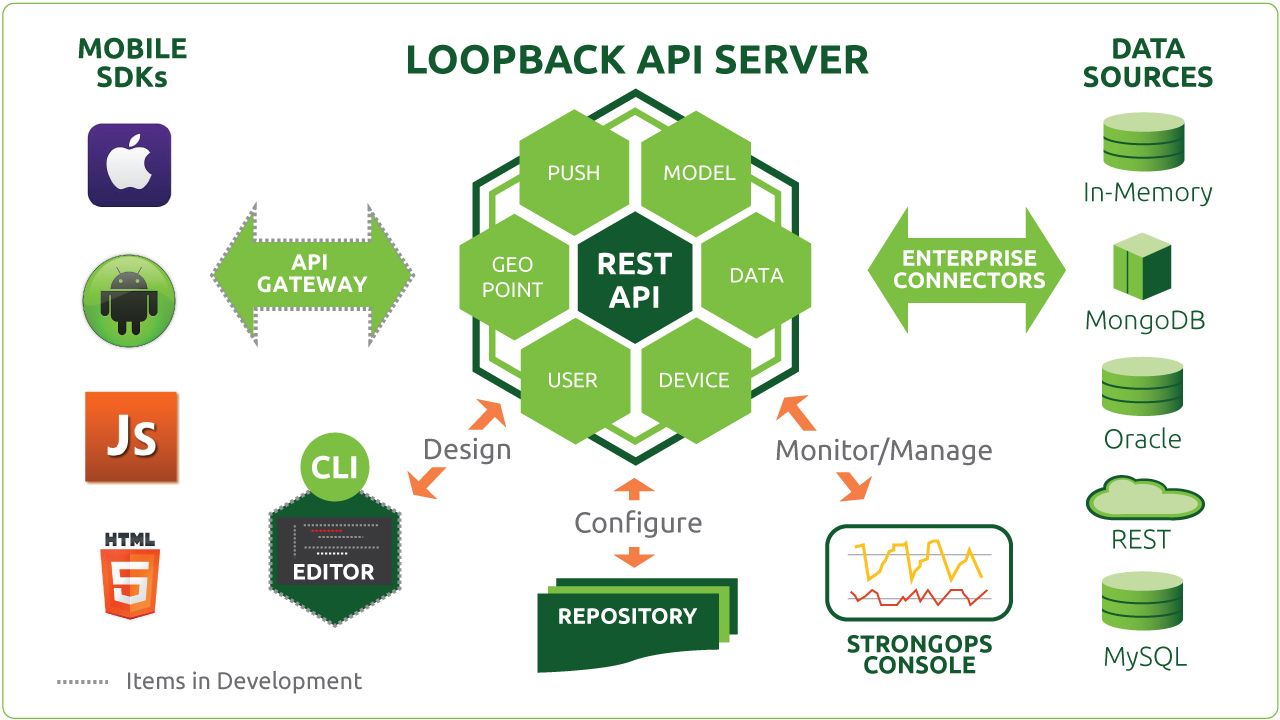
\includegraphics[width=\textwidth]{loopback_1}
\caption{LoopBack Architecture}
\end {figure}



A LoopBack model represents data in backend systems such as databases, and by default has both Node and REST APIs.  Additionally, developer can add functionality such as validation rules and business logic to models.
Every LoopBack application has a set of predefined built-in models such as User, Role, and Application.  Developer can extend built-in models to suit your application's needs.

The model JSON file defines models, relations between models, and access to models. 

\begin{lstlisting}[language=javascript]
{
  "name": "ModelName",  // See Top-level properties below
  "description": "A Customer model representing our customers.",
  "base": "User",
  "idInjection": false,
  "strict": true,
  "options": { ... }, // See Options below
  "properties": { ... }, // See Properties below
  "validations": [...],  // See Validations below
  "relations": {...},  // See Relations below
  "acls": [...],  // See ACLs below
  "scopes": {...},  // See Scopes below
  "http": {"path": "/foo/mypath"}
}
\end{lstlisting}

\subsection{Top-level Properties}

\textbf{Name}

Name of the model.

\textbf{Description}

Optional description of the model.

\textbf{Base}

Name of another model that this model extends. The model will ``inheri'' properties and methods of the base model.

\textbf{IdInjection}

Whether to automatically add an id property to the model:
\begin{itemize}
\item true id property is added to the model automatically. This is the default.
\item false id property is not added to the model.
\end{itemize}

\textbf{Strict}

Specifies whether the model accepts only predefined properties or not. One of:
\begin{itemize}
\item true Only properties defined in the model are accepted. Use if you want to ensure the model accepts only predefined properties.
\item false The model is an open model and accepts all properties, including ones not predefined in the model. This mode is useful to store free-form JSON data to a schema-less database such as MongoDB.
\item validate The unknown properties will be reported as validation errors.
\item throw Throws an exception if properties not defined for the model are used in an operation.
\item Undefined Defaults to false unless the data source is backed by a relational database such as Oracle or MySQL.
\end{itemize}

\textbf{Options}

JSON object that specifies model options.

\textbf{Properties}

JSON object that specifies the properties in the model.

\textbf{Relations}

Object containing relation names and relation definitions.

\textbf{Acls}

Set of ACL specifications that describes access control for the model.

The API can be extended: the developer can add remote functions to mod- els or add hooks to existing API to add custom behavior before and/or after the API handler (to pre-process the re-quest and/or post-process the response). The resulting API is RESTful, cookie free, signed by authentication token. By default, applications have a built-in model that represents a user, with properties username, email and password and role for authentication and authorization. Loopback also introduces an indirection layer that allows to choose from almost all particular DBMS to be used.


\paragraph{}
In Chapter Two the technologies used for developing this work, have been described.
Each technology has been described in realtion to its function and its use in the project.



\chapter{Single Page Application}
\label{cha:chapter_ARC}

This chapter provides an overview of Single Page Application development pattern. First section analyzes the pattern in its totality and provides general and specific definitions. The second section presents pros and cons of the use of Single Page Application, such as SEO problems and speed of load. Third section explains technical functioning of the pattern. 

\section{Section 1}
\label{sec:ARC_section_1}

In this section...

\section{Section 2}
\label{sec:ARC_section_2}

In this section...

\paragraph{}
This chapter has been provided an overview of Single Page Application development pattern. First section has been analyzed the pattern in its totality and provides general and specific definitions. The second section has been presented pros and cons of the use of Single Page Application, such as SEO problems and speed of load. Third section has been explained the technical functioning of the pattern. 



\part{Part 2}
\label{part:part_2}


\chapter{X-Project}
\label{cha:chapter_4}

In questo capitolo verrà presentato la parte principale del progetto di tesi: X-Project.
Nella prima sezione verrà effettuata una panoramica sul progetto, con motivazioni e funzionalità; nella seconda sezione viene fatta una name explanation; nella terza sezione viene presentato un esempio pratico di alcune funzionalità del progetto; nella quarta sezione si mostra l'architettura di X-Project; nella quinta sezione viene esposta la metodologia di sviluppo presentata nel progetto; infine nella sesta e ultima sezione viene presentato un caso d'uso riguardante la creazione di un blog ocn X-Project.


\section{X-Project Overview}
\label{sec:XPR_xpr}

X-Project is a platform to build full-stack Javascript NodeJS API-centric HTML5 based Single Page Application with Web Components via Polymer-Project.
X-Project is composed by guidelines, methodology and a library of elements.
The document driven web development methodology and guidelines allow to build a very structured and usable Single Page Application.

``Everything is an element, even a service'' is the philosophy of the project.

The joint use of Web Components and Strongloop Loopback framework following the document driven web development methodology allowed to create vertical widget that influence every level of the stack. With a descriptive implementation it is possible to give life to API, on the server side, and visual and functional widget on the client side.

A Web Application is essentially built by composing elements together.

The goal of X-Porject is to allow to build a Web Application by composing existing elements. This assumption comes from web application's sharing of essential non-specific components.
Moreover X-Project's goal is to achieve the same easiness of adding an html element, adding logic and function elements.
In fact, in X-Project, an element is a part of the application that comprises both the client side and the server side.

X-Project was born to exploit Web Components benefits and extend them to extreme levels. X-Project, borrows all Web Components and Polymer-Project benefits and adds to them the ones that come from document driven development methodology.
Huge benefits that come from web components environment are reusability and access to reusable code. In fact, by creating stand alone vertical widgets, it's possibile to use components in various forms.
The encapsulation, proper of web components, allows to reuse elements with no concerns of dependencies and specific behaviors.
Benefits of reuse are enhanced by the creation of a set of elements (see \ref{sec:XPR_xel}) that provide a wide range of chances of composition.
This library is composed by a large number of elements of various type: local routing, API, forms, lists, style and page elements. X-Project, according to its philosopy, ``elementize'' everything: local routing elements handle the SPA client-side router (See \ref{sec:ARC_overview}); API elements encapsulate AJAX requests and handle server and database operations; forms, lists and page elements have been created to compose parts and functions of pages; style elements encapsulate group of CSS rules that is applicable to any type of element.


Moreover, thanks to Web Components philosophy and X-Project guidelines, it's easy to gain a clear separation between structure, content, behavior and presentation of elements. 
It's possible to create components that concern the only presentation part of an element, such as mixins in which developers can express groups of CSS rules to be applied to different elements. This aspect also makes style extremly reusable.
In X-Project guidelines this pattern is applied to every kind of element.

Moreover, in the world of web application building platform, there are limits and gaps in terms of ease of use and orientation. As said in \ref{sec:CMS_class}, it is possbile to make a classification of these platforms based on orientation patterns. Nowadays, user oriented platforms have lacks when projects assume big dimensions mainly because of their lack of structure. Developer oriented platforms don't have the same limits, but are defective in ease of use. 



\section{Why the name?}
\label{sec:XPR_name}

The name X-Project has been chosen for three different reasons.
First of all, X character, in maths, can represent every value. Just as this project, the X is variable. X-Project can be used to make any kind of web application, from blogs to e-commerce websites.
So this versatility of mathematical X, fits this project soul.
Secondly, all experimental elements' name created by Google during the dawn of Polymer-Project were preceded by a ``X-'' prefix.
Finally, the X-Project is a sort of a tribute to X-Tag: the Mozilla's web components library \cite{xtag}.


%\section{User Management example: login}
\label{sec:XPR_exmpl}

The example is based on the user login service. 
For this function has been implemented both the client side and the backend. So for the client side has been developed the element \texttt{<form-login>}, for the server side has been developed the element \texttt{<api-user-login>}.

The elements that have been developed are:

\subsubsection{\texttt{<api-user-login>}}

Login a user with the given credentials.

\begin{lstlisting}[language=html]
<api-user-login credentials="{{credentials}}"
collection="{{collection}}" 
response="{{response}}" error="{{error}}"/>
\end{lstlisting}
Where:
\begin{itemize}
\item \texttt{credentials} email and password of user.
\item \texttt{collection} name of collection(Object).
\item \texttt{response}	HTTP response message(String).
\item \texttt{error} object of the error response(Object).
\end{itemize}

\subsubsection{\texttt{<form-login>}}

Create a login form.

\begin{lstlisting}[language=html]
<form id="form" on-submit="on_submit">
    <div class="field">
        <label class="label">email</label>
        <input class="input" is="iron-input" type="text" 
    		placeholder="email" 
            bind-value="{{credentials.email}}">
    </div>
    <div class="field">
        <label class="label">password</label>
        <input class="input" is="iron-input" type="password" 
        	placeholder="password" 
        	bind-value="{{credentials.password}}">
    </div>
      	<input type="submit" value="login"/>
</form>
\end{lstlisting}


\begin {figure}[h]
\graphicspath{{images/chapter_USR/}}

\includegraphics[width=\textwidth]{usr1}
\caption{Login Element Example}
\end {figure}

\section{Media Management example: upload element}
\label{sec:XPR_exmpl_b}

An example of a vertical component is the one that manages media upload on. By introducing a few tags it is possible to handle all the behaviour of the component. In upload case, there is need of only two elements: \texttt{api-upload} and \texttt{part-upload}.
The first one manages the upload functions: server communications and file sending; the second element is a visualization element that shows the input file box and the button ``Choose File''.


The element named \texttt{api-upload} has been designed to upload new files to LocalStorage.
\begin{lstlisting}[language=javascript]
<api-upload id="upload" folder="{{folder}}"
	file="{{file}}" file-name="{{fileName}}">
</api-upload>
\end{lstlisting} 


The element named \texttt{part-upload} has been developed to allow to users to upload new files to LocalStorage.

\begin{lstlisting}[language=javascript]
<api-upload id="upload"
      file="{{file}}" file-name="{{fileName}}">
</api-upload>

<input id="input" type="file" on-change="on_change">
on_change: function () {
      var file = this.$.input.files[0];
      if (!file) {
        return;
      }
      this.fileName = this.fileName || file.name;
      this.file = file;
    }

\end{lstlisting}

The first tag, \texttt{<api-upload>}, set the upload API that handles the request to S3.
The input tag creates a input form that let the user choice the file to upload and trigger the \texttt{on change} function, that send the file via \texttt{<api-upload>} element.



\begin {figure}[h]
\graphicspath{{images/chapter_s3/}}
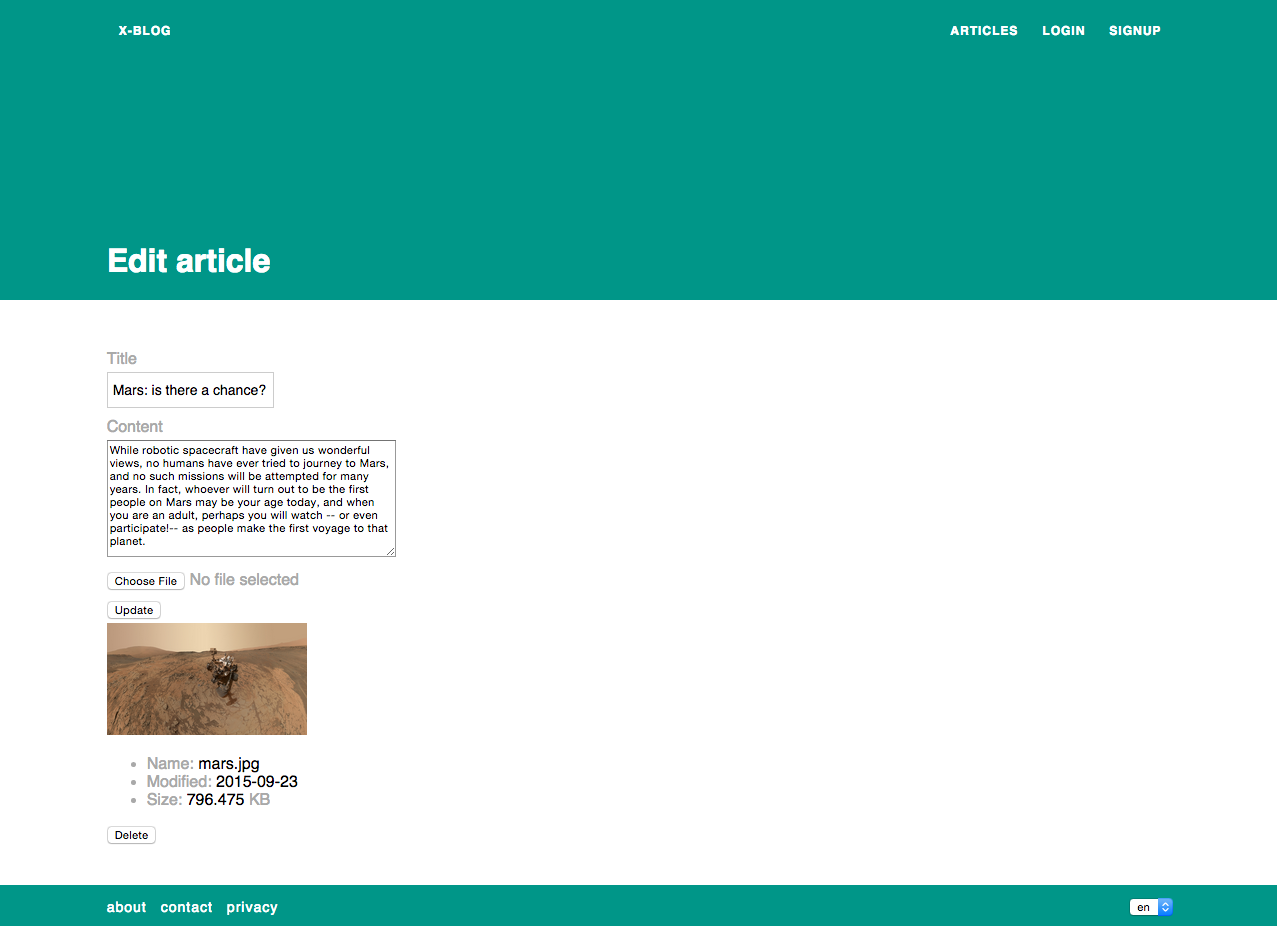
\includegraphics[width=\textwidth]{s3_example}
\caption{Upload component example}
\end {figure}


\section{X-Project Architecture}
\label{sec:XPR_arc}

A Web application developed using the x-project toolkit, an x-project app, is a full stack JavaScript Single Page Application.

Server Side

On the server side, an X-Project app is based on NodeJS (CIT 2.4) used to create the server environment, MongoDB (CIT 2.5) used to storage data, and the Web framework Loopback by Strongloop (CIT 2.6).
Loopback generates model API from the models schemas, to let CRUD operations on models. These schemas are JSON documents.

Client Side

On the client side, an X-Project app is based on HTML5 Web Components via Polymer-Project by Google.
On the top of this stack lies X-Elements a se of Polymer elements for local routing, API request, forms, lists, style and admin pages, as listed further (CIT 4.BOH).

\section{Document-Driven Web Development Process}
\label{sec:XPR_flow}

The process to build a web application based on x-project toolkit consists of the following four steps: models schemas definition, HTTP RESTful API definition, UI components definition and UI components assembly.

\subsection{1st step - Models schemas definition}
\label{sec:XPR_flow_first}
A description of entities, properties, relations and data access policies are defined as JSON documents.

\subsection{2nd step - HTTP RESTful API definition}
\label{sec:XPR_flow_sec}
CRUD operations on models are automatically generated by the web framework (on the basis of input JSON documents) and further custom actions can be defined. All of them are exposed as HTTP RESTful API.

\subsection{3rd step - UI components definition}
\label{sec:XPR_flow_third}
Distinct UI components can be defined, or retrieved from a collection of predefined components, configured and adapted. They represent the building blocks of the whole UI.

\subsection{4th step - UI components assembly}
\label{sec:XPR_flow_third}
Distinct UI components are finally mounted to compose the application views. Assembly is kept as simple as possible: it only consists of a composition of HTML5 elements.
So, the entire development process results driven by: JSON documents describing entities of the application and HTML template documents describing the UI components.



\section{X-Elements}
\label{sec:XPR_xel}

All the following elements are retrievable on a Github repository \cite{xpr_api}.

``Everything is an element'', from an AJAX request to an entire web page. Every part of the website is encapsulated inside an element.

X-project provides a set of Polymer elements for local routing, API requests, forms, lists, style and admin panel, as listed below.

Elements can be customized through their attributes. Attributes can act as inputs parameters (values having effects on the element) or output parameters (values that are returned by the element). Values in parameters could be hard-coded (if they never change) or stored in variables.

Different parameters in different elements could use the same variable, so, the value of an output parameter of an element could be used as input in an input parameter of another element.

\subsection{Elements for local routing}

The following elements perform local routing (for Single Page Application).
\paragraph{\texttt{<x-router>}} Implements local routing using HTML5 Push State API. It represents the core element of the app. It intercepts routes, creates pages, and passes parameters to the page.
\paragraph{\texttt{<x-route>}} Represents a route-to-page mapping. Parameters presented in an URL are sent as attributes to the corresponding page.
\begin{lstlisting}[language=html]
<x-route route="{{route}}" page="{{page}}"/>
\end{lstlisting}
\paragraph{\texttt{<x-link>}} Is an extension of the anchor element <a> that prevents the default behavior when a click event occurs, blocking page request to the server and redirecting the request to the local router.
\begin{lstlisting}[language=html]
<a is="x-link" href="{{href}}">{{link}}/>
\end{lstlisting}

\subsection{Elements for API}

The following elements are used to create API.

\paragraph{\texttt{<api-model-create>}}

Create new instance of Model, and save to database.

\begin{lstlisting}[language=html]
<api-model-create model="{{model}}" data="{{data}}" 
collection="{{collection}}" response="{{response}}" 
error="{{error}}"/>
\end{lstlisting}
Where:
\begin{itemize}
\item \texttt{model} name of model (String)
\item \texttt{data} user data (Object)
\item \texttt{collection} name of collection (Object)
\item \texttt{response}	HTTP response message (String)
\item \texttt{error} object of the error response (Object)
\end{itemize}

\paragraph{\texttt{<api-model-get>}}

Get the id property name of the constructor.

\begin{lstlisting}[language=html]
<api-model-get model_id="{{model_id}}" 
collection="{{collection}}" 
response="{{response}}" error="{{error}}"/>
\end{lstlisting}
Where:
\begin{itemize}
\item \texttt{model-id} id of model (String)
\item \texttt{collection} name of collection (Object)
\item \texttt{response}	HTTP response message (String)
\item \texttt{error} object of the error response (Object)
\end{itemize}

\paragraph{\texttt{<api-model-update>}}

Update multiple instances that match the where clause.

\begin{lstlisting}[language=html]
<api-model-update model_id="{{model_id}} 
"collection="{{collection}}" 
response="{{response}}" error="{{error}}"/>
\end{lstlisting}
Where:
\begin{itemize}
\item \texttt{model-id} id of model(String).
\end{itemize}

\paragraph{\texttt{<api-model-find>}}

Find all model instances that match filter specification.

\begin{lstlisting}[language=html]
<api-model-find where="{{where}} "collection="{{collection}}" 
response="{{response}}" error="{{error}}"/>
\end{lstlisting}
Where:
\begin{itemize}
\item \texttt{where} where clause (Object)
\end{itemize}

\paragraph{\texttt{<api-model-delete>}}

Deletes the model from persistence.

\begin{lstlisting}[language=html]
<api-model-delete model_id="{{model_id}}" 
collection="{{collection}}" 
response="{{response}}" error="{{error}}"/>
\end{lstlisting}
Where:
\begin{itemize}
\item \texttt{model-id} id of model (String)
\end{itemize}

\paragraph{\texttt{<api-model-exists>}}

Check whether a model instance exists in database.

\begin{lstlisting}[language=html]
<api-model-exists model_id="{{model_id}}" exists="{{boolean}}" 
collection="{{collection}}" response="{{response}}" 
error="{{error}}"/>
\end{lstlisting}
Where:
\begin{itemize}
\item \texttt{model-id} id of model (String)
\item \texttt{exists} True if the instance with the specified ID exists; false otherwise (Output)
\end{itemize}

\paragraph{\texttt{<api-model-count>}}

Check whether a model instance exists in database.

\begin{lstlisting}[language=html]
<api-model-count count="{{count}}" collection="{{collection}}" 
response="{{response}}" error="{{error}}"/>
\end{lstlisting}
Where:
\begin{itemize}
\item \texttt{count} number of instances updated (Output)
\end{itemize}

\subsection{Elements for forms}

The following elements are used to create forms.

\paragraph{\texttt{<x-input>}} 

Is an extension of the input element.
\begin{lstlisting}[language=html]
<x-input type="{{type}}" label="{{label}}" value="{{value}}"/>
\end{lstlisting}
Where:
\begin{itemize}
\item \texttt{type} can be string, number, date, email, url, location (with auto-completion based on Google Place API) and file.
\end{itemize}

\paragraph{\texttt{<x-form>}} Dynamically generates a form from a model schema, to create/update a model.
\begin{lstlisting}[language=html]
<x-form schema="{schema}" model="{model}"/>
\end{lstlisting}

\subsection{Elements for lists}

The following elements are used to manage lists.

\paragraph{\texttt{<x-table>}} Dynamically generates a table of models from a model schema.
\begin{lstlisting}[language=html]
<x-table schema="{{schema}}" items="{{items}}"/>
\end{lstlisting}
Where:
\begin{itemize}
\item \texttt{schema} is used to generate the columns of the table. 
\item \texttt{items} is used to generate the rows (the values) of the table.
\end{itemize}

\paragraph{\texttt{<x-pager>}} Generates the list of links to handle pagination.
\begin{lstlisting}[language=html]
<x-pager perpage="{{perpage}}" count="{{count}}" 
current="{{page}}"/>
\end{lstlisting}
Where:
\begin{itemize}
\item \texttt{count} is the total number of items to paginate.
\item \texttt{perpage} is the number of items per page.
\item \texttt{current} is the current page selected by the user.
\end{itemize}

By itself pagination doesn’t paginate any list, but it can be used in conjunction with <api-collection-get> (as shown in the case study), where the current output parameter of <x-pager> is the input page parameter of  <api-collection-get>.


\subsection{Elements for style}

The style is based on iron-flex-layout, a CSS library of style mixins for cross-platform Flexible Box layouts.

\subsection{Elements for admin panel}

Even a page can be encapsulated in an element. x-project provides a set of pages for the admin part of the app, <page-collection> and <page-model-edit>, presented below.

\subsection{Elements for pages}

\paragraph{\texttt{<x-header>}} This element is used to insert an header at the top of the page.
\begin{lstlisting}[language=html]
<x-header links="{{links}}" brand="{{brand}}"/>
\end{lstlisting}
Where:
\begin{itemize}
\item \texttt{links} is the total number of items to paginate.
\item \texttt{brand} is the number of items per page.
\end{itemize}
\paragraph{\texttt{<x-footer>}} This element is used to insert an footer at the botton of the page.
\begin{lstlisting}[language=html]
<x-footer links="{{links}}" notes="{{notes}}"/>
\end{lstlisting}
Where:
\begin{itemize}
\item \texttt{links} is the total number of items to paginate.
\item \texttt{notes} is the number of items per page.
\end{itemize}
\paragraph{\texttt{<x-crew>}} This element is used to insert the section for the presentation of the team of a project.
\begin{lstlisting}[language=html]
<x-crew team="{{team}}"/>\end{lstlisting}
Where:
\begin{itemize}
\item \texttt{team} is the total number of items to paginate.
\end{itemize}
\paragraph{\texttt{<x-contact>}}This element is used to insert the section for the presentation of the contact.
\begin{lstlisting}[language=html]
<x-contact contact="{{contact}}"/>\end{lstlisting}
Where:
\begin{itemize}
\item \texttt{links} is the total number of items to paginate.
\item \texttt{brand} is the number of items per page.
\end{itemize}


\paragraph{}
In this chapter has been described the main part of thesis project: X-Project.
First of all it has been provided an overview of the project, later it has been introduced a name explaination. In the last sections has been introduced X-Project architecture, its functionality and in conclusion have been presented some elements.



\chapter{Media Management: Amazon S3 Component}
\label{cha:chapter_S3}

In this chapter...

\section{Amazon AWS}
\label{sec:s3_aws}

Amazon Web Services (AWS), a collection of remote computing services, also called web services, make up a cloud-computing platform offered by Amazon.com.\cite{aws_overview} These services operate from 11 geographical regions across the world. The most central and well-known of these services arguably include Amazon Elastic Compute Cloud and Amazon S3. Amazon markets these products as a service to provide large computing-capacity more quickly and more cheaply than a client company building an actual physical server farm \cite{aws_cloud}.

AWS is located in 11 geographical ``regions'': US East (Northern Virginia), where the majority of AWS servers are based,\cite{aws_stats1} US West (northern California), US West (Oregon), Brazil (São Paulo), Europe (Ireland and Germany), Southeast Asia (Singapore), East Asia (Tokyo and Beijing) and Australia (Sydney). There is also a ``GovCloud'', based in the Northwestern United States, provided for U.S. government customers, complementing existing government agencies already using the US East Region.[4] Each Region is wholly contained within a single country and all of its data and services stay within the designated Region.[citation needed]

Each Region has multiple ``Availability Zones'', which are distinct data centers providing AWS services. Availability Zones are isolated from each other to prevent outages from spreading between Zones. Several services operate across Availability Zones (e.g., S3, DynamoDB) while others can be configured to replicate across Zones to spread demand and avoid downtime from failures. Amazon web services hold 1.79\% market share. As of December 2014, Amazon Web Services operated an estimated 1.4 Million servers across 28 availability zones \cite{aws_stats2}.

\section{Amazon S3}
\label{sec:s3_s3}

Amazon S3 (Simple Storage Service) is an online file storage web service offered by Amazon Web Services. Amazon S3 provides storage through web services interfaces (REST, SOAP, and BitTorrent).Amazon launched S3, its first publicly available web service, in the United States in March 2006 and in Europe in November 2007 \cite{s3_overview}.

Amazon S3 is reported to store more than 2 trillion objects as of April 2013.\cite{s3_stats} S3 uses include web hosting, image hosting, and storage for backup systems. 
Amazon S3 provides an API (Application programming interface) for third-party developers. It describes various API operations, related request and response structures, and error codes.[38] Web services interface can be used to store and retrieve any amount of data, at any time, from anywhere on the web. It gives any developer access to the same highly scalable, reliable, secure, fast, inexpensive infrastructure that Amazon uses to run its own global network of web sites. The service aims to maximize benefits of scale and to pass those benefits on to developers. Today there are different kinds of file managers for Amazon S3. An effective solution for Amazon provides a user interface to Amazon S3 accounts, files and buckets, allowing to browse, create and delete files and buckets.[39]

\section{CORS}
\label{subsec:S3_cors}

Cross-origin resource sharing (CORS) is a mechanism that allows restricted resources (e.g. fonts, JavaScript, etc.) on a web page to be requested from another domain outside the domain from which the resource originated.

A web page may freely embed images, stylesheets, scripts, iframes, videos and some plugin content (such as Adobe Flash) from any other domain. However embedded web fonts and AJAX (XMLHttpRequest) requests have traditionally been limited to accessing the same domain as the parent web page (as per the same-origin security policy).``Cross-domain'' AJAX requests are forbidden by default because of their ability to perform advanced requests (POST, PUT, DELETE and other types of HTTP requests, along with specifying custom HTTP headers) that introduce many cross-site scripting security issues.

CORS defines a way in which a browser and server can interact to safely determine whether or not to allow the cross-origin request. It allows for more freedom and functionality than purely same-origin requests, but is more secure than simply allowing all cross-origin requests. It is a recommended standard of the W3C.

The CORS standard describes new HTTP headers which provide browsers and servers a way to request remote URLs only when they have permission. Although some validation and authorization can be performed by the server, it is generally the browser's responsibility to support these headers and respect the restrictions they impose.

For AJAX and HTTP request methods that can modify data (usually HTTP methods other than GET, or for POST usage with certain MIME types), the specification mandates that browsers ``preflight'' the request, soliciting supported methods from the server with an HTTP OPTIONS request header, and then, upon ``approval'' from the server, sending the actual request with the actual HTTP request method. Servers can also notify clients whether ``credentials'' (including Cookies and HTTP Authentication data) should be sent with requests \cite{s3_cors}. 

\begin {figure}[h]
\graphicspath{{images/chapter_s3/}}
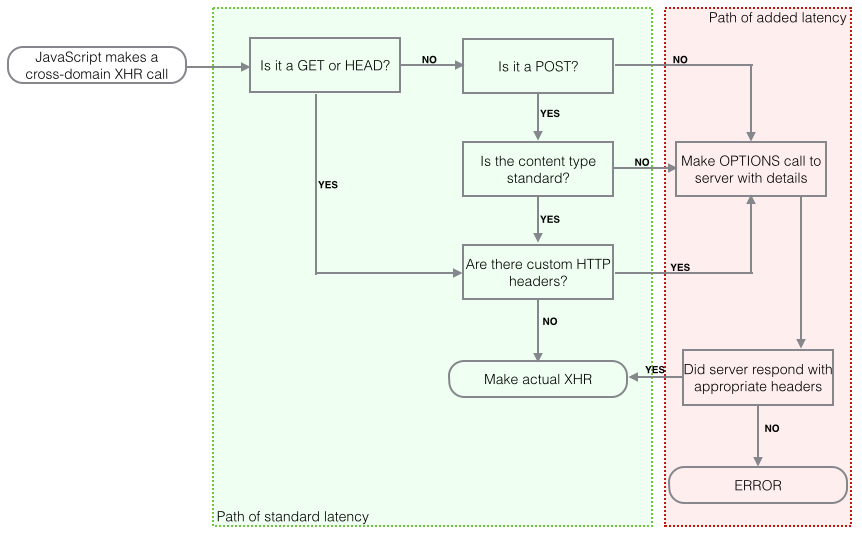
\includegraphics[width=\textwidth]{cors}
\caption{Flowchart showing Simple and Preflight XHR by Bluesmoon}
\end {figure}



\section{Media Management S3 Component}
\label{sec:S3_component}

In this section will be analyzed the Media Management S3 Component, developed to store images and documents on cloud through Amazon S3 Service.
This specific component has been developed in order to store and manage media files in Amazon S3 service.
Operations that can be done, like upload, delete or get media, is ruled by CORS (\ref{subsec:S3_cors}) pattern.
These operations are direct: none of them is done via server. Server is only used to get the authorization to communicate with the S3 cloud storage service.
In fact, client makes an AJAX request to server in order to get the Signed URL, that is the request URL combined with the name of S3 Bucket and the dedicated Region.
The Signed URL pattern represents the Digital Signature security mechanism, as seen in \ref{sec:digsign}.

The Signed URL is requested via an ad hoc API, that is exposed to client side through a remote method.
Get, Upload and Delete functions have been implemented on the server side using an additional library named AWS SDK for Javascript NodeJS \footnote{ The AWS SDK helps take the complexity out of coding by providing JavaScript objects for AWS services including Amazon S3, Amazon EC2, DynamoDB, and Amazon SWF.} \cite{s3_aws_sdk}.

Each function create a request for a Signed URL to its server.
Using file's name, bucket's name, bucket's region and user key, the server gives back an URL to which the client can his real HTTP request.

Once the client receive the Signed URL can pass the operation to S3 Service and carry it out.
Bucket and Region names are stored in \texttt{.env} file and must be set up before on S3 website.
Moreover, users must set Bucket's CORS Configuration on S3 Admin Panel (as shown in fig. \ref{s3panel}): CRUD operations must be allowed from the user in the CORS Configuration Editor panel.


\paragraph{Upload Signed Url Request}

\begin{lstlisting}[language=javascript]
Image.signed_put = function(file_name, file_type, callback) {
    var s3 = new aws.S3();
    var s3_params = {
      Bucket: S3_BUCKET,
      Key: file_name,
      Expires: 60,
      ContentType: file_type,
      ACL: 'public-read'
    };
    s3.getSignedUrl('putObject', s3_params,
     function (err, signed_url) {
      if (err) {
        callback(err);
        return;
      }
      callback(null, signed_url);
    });
  };

  Image.remoteMethod('signed_put', {
    http: { verb: 'get' },
    accepts: [
      {arg: 'file_name', type: 'string'},
      {arg: 'file_type', type: 'string'}
    ],
    returns: {arg: 'signed_url', type: 'string'}
  });
\end{lstlisting}

\paragraph{Get Signed Url Request}

\begin{lstlisting}[language=javascript]
Image.signed_list = function (folder, callback) {
    var s3 = new aws.S3();
    var s3_params = {
      Bucket: S3_BUCKET,
      EncodingType: 'url',
      Prefix: folder,
      MaxKeys: 1000
    };
    s3.getSignedUrl('listObjects', s3_params,
     function (err, signed_url) {
      if (err) {
        callback(err);
        return;
      }
      callback(null, signed_url);
    });
  };

  Image.remoteMethod('signed_list', {
    http: { verb: 'get' },
    accepts: { arg: 'folder', type: 'string' },
    returns: { arg: 'signed_url', type: 'string' }
  });
\end{lstlisting}


\paragraph{Delete Signed Url Request}

\begin{lstlisting}[language=javascript]
Image.signed_delete = function(file_name, callback) {
    var s3 = new aws.S3();
    var s3_params = {
      Bucket: S3_BUCKET,
      Key: file_name
    };
    s3.getSignedUrl('deleteObject', s3_params,
      function (err, signed_url) {
      if (err) {
        callback(err);
        return;
      }
      callback(null, signed_url);
    });
  };

  Image.remoteMethod('signed_delete', {
    http: { verb: 'get' },
    accepts: {arg: 'file_name', type: 'string'},
    returns: {arg: 'signed_url', type: 'string'}
  });

\end{lstlisting}


\begin {figure}[h]
\graphicspath{{images/chapter_s3/}}
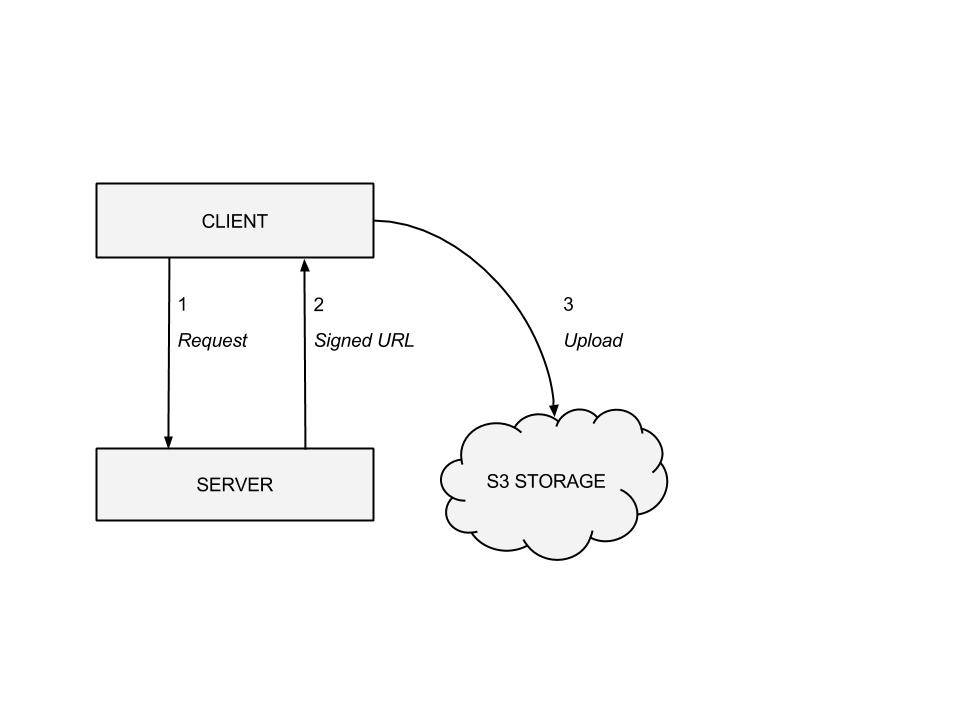
\includegraphics[width=\textwidth]{s3_upload}
\caption{S3 direct upload process}
\end {figure}



\begin {figure}[h]
\graphicspath{{images/chapter_s3/}}
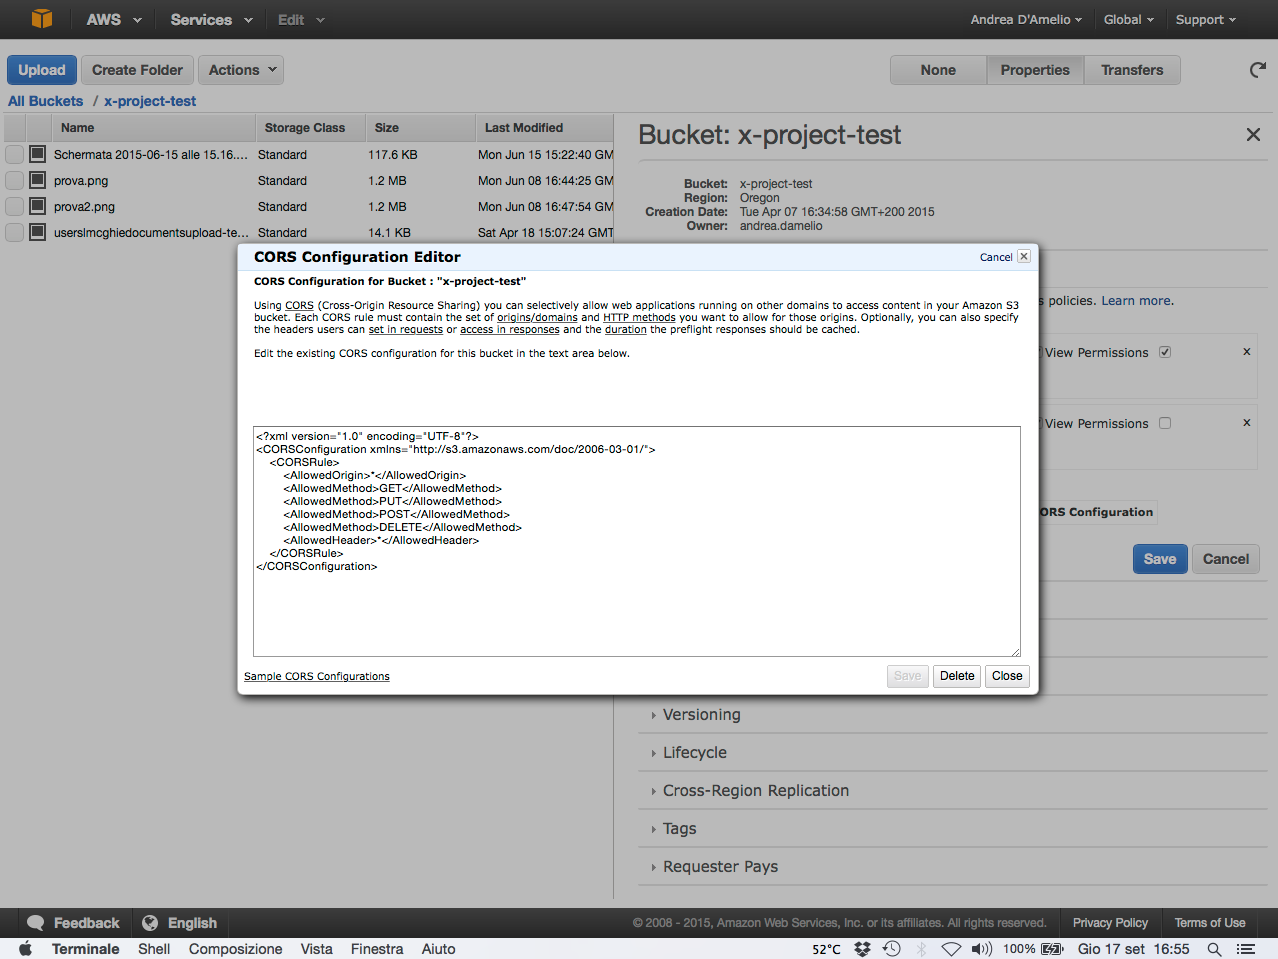
\includegraphics[width=\textwidth]{s3panel}
\caption{S3 CORS Configuration Editor Panel}
\end {figure}









\subsection{S3 Component Elements}
\label{subsec:S3_server_elem}


In order to use Media Management S3 Component in an X-Project App there's need to combinate six different X-Elements:
\begin{itemize}

\item\texttt{api-s3-upload},
\item\texttt{api-s3-list},
\item\texttt{api-s3-delete},
\item\texttt{part-s3-list},
\item\texttt{part-s3-list-item}
\item\texttt{part-s3-upload}.

\end{itemize}

Each element provides the opportunity to use one of the basic function of Amazon S3 service. 

\subsubsection{\texttt{api-s3-upload}}
\label{api-s3-upload}


The element named \texttt{api-s3-upload} has been designed to upload new files to the S3 Bucket.
\begin{lstlisting}[language=javascript]
<api-s3-upload id="upload" folder="{{folder}}"
	file="{{file}}" file-name="{{fileName}}">
</api-s3-upload>
\end{lstlisting}


\subsubsection{\texttt{api-s3-list}}
\label{api-s3-list}
The element named \texttt{api-s3-list} has been designed to get the list of elements currently in the S3 Bucket.
\begin{lstlisting}[language=javascript]
<api-s3-list id="list" list="{{list}}">
</api-s3-list>
\end{lstlisting}


\subsubsection{\texttt{api-s3-delete}}
\label{api-s3-delete}
The element named \texttt{api-s3-delete} has been designed to delete an element currently in the S3 Bucket.
\begin{lstlisting}[language=javascript]
<api-s3-delete id="request" file-name="{{item.key}}">
</api-s3-delete>
\end{lstlisting}


\subsubsection{\texttt{part-s3-list}}
\label{part-s3-list}
The element named \texttt{part-s3-list} has been developed to show the list of elements currently in the S3 Bucket
\begin{lstlisting}[language=html]
<template>
    <api-s3-list id="list" list="{{list}}">
    </api-s3-list>

    <template is="dom-repeat" items="{{list}}" filter="filter">
        <part-s3-list-item item="{{item}}" on-delete="update">
        </part-s3-list-item>
    </template>
</template>
\end{lstlisting}
The first tag, \texttt{<api-s3-list>}, calls the GET API that handles the request to S3, and returns the list of elements currently in S3 Bucket.
The second tag, \texttt{<part-s3-list-item>}, creates a visual element for each object currently in the bucket. This cycle is expressed via the attribute \texttt{``dom-repeat''}.


\subsubsection{\texttt{part-s3-list-item}}
\label{part-s3-list-item}
The element named \texttt{part-s3-list-item} has been developed to show a preview of a selected files and to let the user delete it.
\begin{lstlisting}[language=javascript]

 <api-s3-delete id="request" file-name="{{item.key}}">
 </api-s3-delete>
 ...
 <button id="delete" on-click="delete_image">delete
 </button>
 ...
 delete_image: function () {
      this.$.request.send();
 }
 ...
\end{lstlisting}

The first tag, \texttt{<api-s3-delete>}, set the DELETE API that handles the request to S3.
The button tag creates a button that, when clicked, trigger the \texttt{delete image} function, that makes the call via \texttt{<api-s3-delete>} element.


\subsubsection{\texttt{part-s3-upload}}
\label{part-s3-upload}
The element named \texttt{part-s3-upload} has been developed to allow to users to upload new files to the S3 Bucket.

\begin{lstlisting}[language=javascript]
<api-s3-upload id="upload"
      file="{{file}}" file-name="{{fileName}}">
</api-s3-upload>

<input id="input" type="file" on-change="on_change">
on_change: function () {
      var file = this.$.input.files[0];
      if (!file) {
        return;
      }
      this.fileName = this.fileName || file.name;
      this.file = file;
    }

\end{lstlisting}

The first tag, \texttt{<api-s3-upload>}, set the UPLOAD API that handles the request to S3.
The input tag creates a input form that let the user choice the file to upload and trigger the \texttt{on change} function, that send the file via \texttt{<api-s3-upload>} element.


In conclusions...



\chapter{User Management: Login toolkit}
\label{cha:chapter_USR}

In this chapter...

\section{User Management Component}
\label{sec:USR_user_management}

The application list addressed to a community of users / customers have to implement the management mechanisms of the user.

The mechanisms for base user management are:
\begin{itemize}
\item user login 
\item user signup
\item user logout
\item user management
\end{itemize}
To these advanced management mechanism may be associated, such as:
\begin{itemize}
\item email verification 
\item email changing  
\item password recovery/reset 
\item password changing  
\end{itemize}

The mechanisms of advanced management, involving the use of email, must necessarily be based on a email management service.
Challenge of this project is to be able to encapsulate these mechanisms / behaviors in their elements, to allow it to integrate user management with the same ease with which it is possible to insert HTML elements on a page.

\subsection{User Management services}
\label{subsec:USR_user_management_services}
This section talks about the various existing services for user management as: Stormpath, Userapp and Auth0.
\subsubsection{Stormpath}

Stormpath is a User Management API that reduces development time with instant-on, scalable user infrastructure. Stormpath's intuitive API and expert support make it easy for developers to authenticate, manage and secure users and roles in any application.

Stormpath,it has a simple goal: give developers a complete user management system, so can focus on building great applications.\cite{usr_stormpath}

\begin{itemize}
\item Pre-built authentication \& authorization.
\item Schemaless, secure user data \& profiles.
\item Code-free Active Directory, Facebook \& Google login.
\item Open Source SDKs \& complete sample apps.
\end{itemize}

\begin {figure}[h]
\graphicspath{{images/chapter_USR/}}
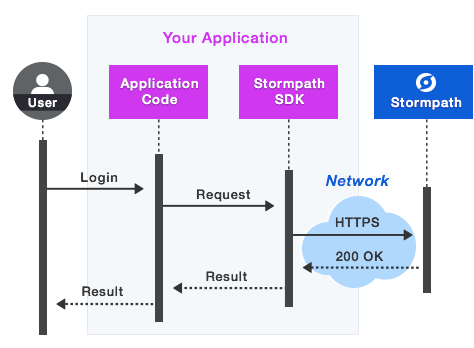
\includegraphics[width=\textwidth]{stormpath}
\caption{Stormpath User Management API}
\end {figure}

\subsubsection{Userapp}

UserApp is a cloud-based user management API for web apps. The purpose is to relieve developers from having to program logic for login, sign up, calculate payments, turn on or off features, etc. And instead focus on their core product.

UserApp provides with user management functionality that results in faster development, faster revenue, more users, and the ability to serve users better by engaging with them more efficiently.\cite{usr_userapp}

\begin{itemize}
\item User authentication - Have the user authentication ready today. It is possible just a few lines of code away with one of SDKs.
\item One-click integrations - Integrate the users with third-party services with just one click.
\item Mobile, web, and server - No matter where is need to integrate the user authentication, it got  covered.
\end{itemize}

\subsubsection{Auth0}

Auth0 is an enterprise-grade platform for modern identity.
Auth0 give the tools that eliminate the friction of authentication for the applications and APIs - all accessible through the account dashboard.\cite{usr_auth0}

\begin {figure}[h]
\graphicspath{{images/chapter_USR/}}
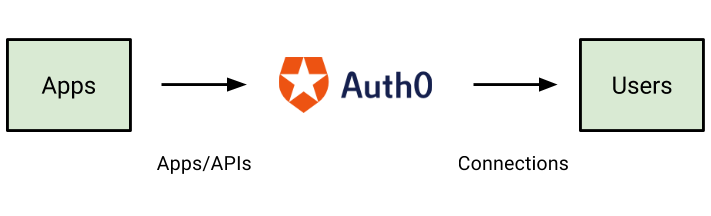
\includegraphics[width=\textwidth]{auth0}
\caption{Auth0 Overview}
\end {figure}

It is possible connect any application, written on any language or stack to Auth0, and separately define how users of that application authenticate:

\begin{itemize}
\item Custom credentials: username/passwords.
\item Social network logins: Google, Facebook, Twitter and any OAuth2 or OAuth1 provider.
\item Enterprise directories: LDAP, Google Apps, Office 365, ADFS, AD, SAML-P, WS-Federation, etc.,
\item Password-less systems: TouchID, one time codes on SMS.
\end{itemize}


\subsection{User Management standard API in LoopBack}

X-project is based on StrongLoop LoopBack on the server side.
LoopBack's built-in User model provides essential user management features such as:
\begin{itemize}
\item Registration and confirmation via email.
\item Login and logout.
\item Creating an access token.
\item Password reset. 
\end{itemize}
In general can extend the User model to suit specific needs, so in most cases, it is don't need to create the own User model from scratch.
By default, a LoopBack application has a built-in User model defined by user.json
In particular, it was implemented the connection with MailChimp service, named Mandrill.

\subsection{User Management remote methods}

In addition to the standard APIs, remote methods for email and password changing have been implemented. 

\subsubsection{Change Email}

\begin{lstlisting}[language=html]
Author.change_email = function (new_email, confirm_email, password, cb) {
    if (new_email !== confirm_email) {
      cb({ error: 'email not confirmed' }, null);
      return;
    }

    var userId = getCurrentUserId();  

    Author.findById(userId, function (err, user) {
      if (err) {
        cb(err, null);
        return;
      }

      user.hasPassword(password, function (err, match) {
        if (!match) {
          cb({ error: 'invalid password' }, null);
          return;
        }

        user.updateAttribute('email', new_email, function (err, user) {
          if (err) {
            cb(err, null);
            return;
          }

          cb(null, true);
        });
	  });       
	});
};
   Author.remoteMethod('change_email', {
    http: { path: '/change_email', verb: 'post' },
    accepts: [
      { arg: 'new_email', type: 'string' },
      { arg: 'confirm_email', type: 'string' },
      { arg: 'password', type: 'string' }
    ],
    returns: { arg: 'changed', type: 'boolean' }
  });
\end{lstlisting}

\subsubsection{Change Password}

\begin{lstlisting}[language=html]
Author.change_password = function (new_password, confirm_password, password, cb) {
    if (new_password !== confirm_password) {
      cb({ error: 'password not confirmed' }, null);
      return;
    }

    var userId = getCurrentUserId();  

    Author.findById(userId, function (err, user) {
      if (err) {
        cb(err, null);
        return;
      }

      user.hasPassword(password, function (err, match) {
        if (!match) {
          cb({ error: 'invalid password' }, null);
          return;
        }

        user.updateAttribute('password', new_password, function (err, user) {
          if (err) {
            cb(err, null);
            return;
          }

          cb(null, true);
        });
	  });       
    });
  };
   
  Author.remoteMethod('change_password', {
    http: { path: '/change_password', verb: 'post' },
    accepts: [
      { arg: 'new_password', type: 'string' },
      { arg: 'confirm_password', type: 'string' },
      { arg: 'password', type: 'string' }
    ],
    returns: { arg: 'changed', type: 'boolean' }
  });
\end{lstlisting}




\section{User Managament elements}

Some elements have been created for user managment.
Both style and behavior of these elements have been developed , so that every user can easily customize it at will and choose to use either one side or both sides of the element.
The main elements are the ones developed for the management as: login, logout, signup and reset.
The specifications for each element are indicated below.

\subsubsection{\texttt{<api-user-login>}}

Login a user with the given credentials.
\begin{lstlisting}[language=html]
<api-user-login credentials="{{credentials}}"
collection="{{collection}}" 
response="{{response}}" error="{{error}}"/>
\end{lstlisting}
Where:
\begin{itemize}
\item \texttt{credentials} email and password of user.
\item \texttt{collection} name of collection(Object).
\item \texttt{response}	HTTP response message(String).
\item \texttt{error} object of the error response(Object).
\end{itemize}

\begin {figure}[h]
\graphicspath{{images/chapter_USR/}}

\includegraphics[width=\textwidth]{usr1}
\caption{Login Element}
\end {figure}

\subsubsection{\texttt{<api-user-logout>}}

Logout a user with the given accessToken id.
\begin{lstlisting}[language=html]
<api-user-logout collection="{{collection}}" 
response="{{response}}" error="{{error}}"/>
\end{lstlisting}
Where:
\begin{itemize}
\item \texttt{credentials} email and password of user.
\item \texttt{collection} name of collection (Object)
\item \texttt{response}	HTTP response message (String)
\item \texttt{error} object of the error response (Object)
\end{itemize}

\subsubsection{\texttt{<api-user-signup>}}

Signup a user by with the given general information.
\begin{lstlisting}[language=html]
<api-user-signup credentials="{{credentials}}"
collection="{{collection}}" 
response="{{response}}" error="{{error}}"/>
\end{lstlisting}
Where:
\begin{itemize}
\item \texttt{credentials} email, password, name and phone-number of user.
\item \texttt{collection} name of collection (Object)
\item \texttt{response}	HTTP response message (String)
\item \texttt{error} object of the error response (Object)
\end{itemize}

\begin {figure}[h]
\graphicspath{{images/chapter_USR/}}

\includegraphics[width=\textwidth]{usr4}
\caption{Signup Element}
\end {figure}

\subsubsection{\texttt{<api-user-reset>}}

Create a short lived acess token for temporary login. Allows users to change passwords if forgotten.
\begin{lstlisting}[language=html]
<api-user-reset email="{{email}}"
collection="{{collection}}" 
response="{{response}}" error="{{error}}"/>
\end{lstlisting}
Where:
\begin{itemize}
\item \texttt{email} email of user (String)
\item \texttt{collection} name of collection (Object)
\item \texttt{response}	HTTP response message (String)
\item \texttt{error} object of the error response (Object)
\end{itemize}

\begin {figure}[h]
\graphicspath{{images/chapter_USR/}}

\includegraphics[width=\textwidth]{usr3}
\caption{Reset Element}
\end {figure}

\begin {figure}[h]
\graphicspath{{images/chapter_USR/}}

\includegraphics[width=\textwidth]{usr4}
\caption{Login Element}
\end {figure}

\subsubsection{\texttt{<form-login>}}

Create a login form.
\begin{lstlisting}[language=html]
<form id="form" on-submit="on_submit">
    <div class="field">
        <label class="label">email</label>
        <input class="input" is="iron-input" type="text" 
    		placeholder="email" 
            bind-value="{{credentials.email}}">
    </div>
    <div class="field">
        <label class="label">password</label>
        <input class="input" is="iron-input" type="password" 
        	placeholder="password" 
        	bind-value="{{credentials.password}}">
    </div>
      	<input type="submit" value="login"/>
</form>
\end{lstlisting}

\subsubsection{\texttt{<form-signup>}}

Create a signup form.
\begin{lstlisting}[language=html]
<form id="form" on-submit="on_submit">
    <div class="field">
        <label class="label">email</label>
        <input class="input" is="iron-input" type="text" 
    		placeholder="email" 
            bind-value="{{credentials.email}}">
    </div>
    <div class="field">
        <label class="label">password</label>
        <input class="input" is="iron-input" type="password" 
        	placeholder="password" 
        	bind-value="{{credentials.password}}">
    </div>
    <div class="field">
        <label class="label">firstname</label>
        <input class="input" is="iron-input" type="text" 
        	placeholder="firstname" 
        	bind-value="{{credentials.firstname}}">
    </div>
    <div class="field">
        <label class="label">lastname</label>
        <input class="input" is="iron-input" type="text" 
        	placeholder="lastname" 
        	bind-value="{{credentials.lastname}}">
    </div>
    <div class="field">
        <label class="label">phone-number</label>
        <input class="input" is="iron-input" type="text" 
        	placeholder="phone-number" 
        	bind-value="{{credentials.phone-number}}">
    </div>
      	<input type="submit" value="confirm"/>
</form>
\end{lstlisting}


\subsubsection{\texttt{<form-reset>}}

Create a reset form.
\begin{lstlisting}[language=html]
<form id="form" on-submit="on_submit">
    <div class="field">
        <label class="label">email</label>
        <input class="input" is="iron-input" type="text" 
    		placeholder="email" 
            bind-value="{{credentials.email}}">
    </div>
      	<input type="submit" value="reset"/>
</form>
\end{lstlisting}

\subsubsection{User Settings}

The User Settings is the page where it is possible to manage the personal data such as e-mail and password.

\begin {figure}[h]
\graphicspath{{images/chapter_USR/}}
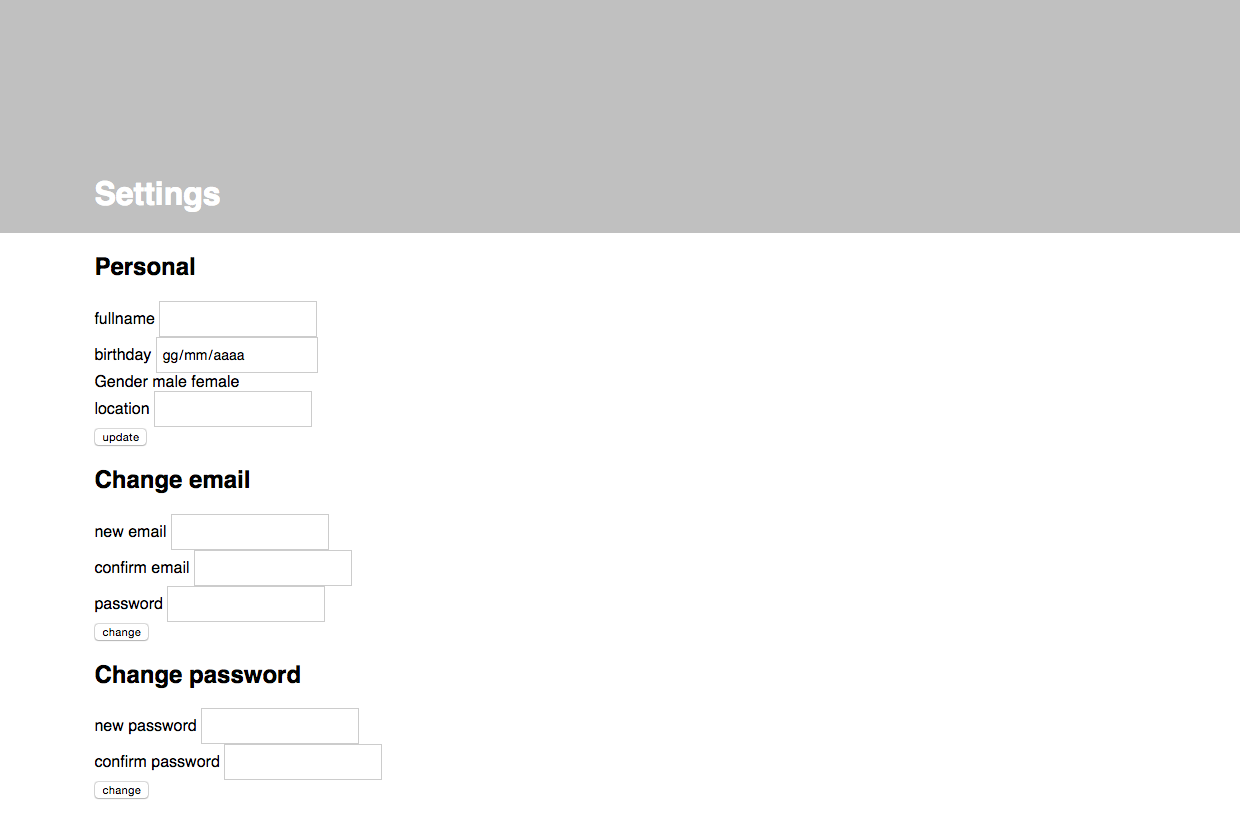
\includegraphics[width=\textwidth]{usr2}
\caption{Settings  Element}
\end {figure}


\section{Mandrill}
\label{sec:USR_mandrill}


Mandrill is a reliable, scalable, and secure delivery API for transactional emails from websites and applications. It's ideal for sending data-driven transactional emails, including targeted e-commerce and personalized one-to-one messages.
Trusted by more than 500,000 customers, Mandrill runs on a globally distributed infrastructure that can deliver emails in milliseconds.
Mandrill was developed by MailChimp, a company with more than 10 years of experience building a robust email marketing platform. MailChimp sends 15 billion emails every month for more than 8 million customers.


\subsubsection{Mailchimp}
\label{subsubsec:USR_mandrill_mailchimp}
MailChimp is an email marketing service and trading name of its operator, a United States company, founded in 2001.
The MailChimp service is accessed through a web- or mobile-based application; for some features there is an offline application.
MailChimp began as a paid service and added a freemium option eight years later.[5] It was originally going to be called ChimpMail, but the name was changed after the company discovered that they could not get that domain name.
The company's logo is a chimpanzee, and the site includes numerous chimp-related graphics and humor on its website and in its communications.

\paragraph{}
In this chapter, the general characteristics of the component have been presented for user management.
This component allows developers to integrate into their application functions required for managing user as login or signup.

This element lets the developers to integrate in applications important user management fuctions, such as login and signup.
In particular Mailchimp service has been used for development and management of signup and reset password.



\chapter{Caso d'uso: X-Journal}
\label{cha:chapter_CAS}

This chapter presents a use case of the project, the implementation of a blog via X-Project toolkit.
Sections provides the rappresentation of elements equipped with several code snippets and examples.


\section{Case Study}
\label{sec:CAS_castudy}

In this section the design and the implementation of a blog platform is presented.

\subsection{1st step - Models schemas definition}

As to a blog platform, the essential entities to be modelled are the following: Post and Tag.

\begin{lstlisting}[language=javascript]
{
	"name": "Post",
	"properties": {
		"title": {"type":"string"},
		"posted": {"type":"date"},
		"content": {"type":"text"},
		"permalink": {"type":"string"}
	},
	"relations": {
		"tags": {"type":"has_many","model":"Tag"}
	}
}
\end{lstlisting}

\begin{lstlisting}[language=javascript]
{
	"name": "Tag",
	"properties": {
		"name": {"type":"string"}
	}
}
\end{lstlisting}

\subsection{2nd step - HTTP RESTful API definition}

These models result in the following HTTP RESTful API, automatically generated by Loopback server.

\begin{lstlisting}[language=javascript]
	GET / api / Posts
	POST / api / Posts
	GET / api / Posts /: post_id
	PUT / api / Posts /: post_id
	DELETE / api / Posts /: post_id
	GET / api / Tags
	POST / api / Tags
	GET / api / Tags /: tag_id
	PUT / api / Tags /: tag_id
	DELETE / api / Tags /: tag_id
\end{lstlisting}

\subsection{3rd step - UI components definition}

In this simple example, there is no need to define further components besides the ones provided by the x-project toolkit.

\subsection{4th step - UI components assembly}

Since a snippet is worth a thousand words, in the following the code of the pages of the app is shown. It is important to remark how easily a page can be built without writing code but assembling elements.

Tha admin part is composed by page-collection and page-model-edit. These pages are accessible via the following routes.

\begin{lstlisting}[language=html]
<x-router>
	<x-route route="/admin/:collection"page="page-collection"/>
	<x-route route="/admin/:collection/:id"page="page-model-edit"/>
</x-router>
\end{lstlisting}

Where: the parameter :collection is the name of the collection to inspect; the parameter :id is the id of the model to edit. These parameters are set as attributes of the page element.

\begin{itemize} \texttt{<page-collection>} Shows the models of a collection.

\begin{lstlisting}[language=html]
<template name= "page-collection">
	<api-collection-schema name="{{collection}}" 
	schema="{{schema}" />
	<api-collection-get name="{{collection}}" 
	where="{{where}}" page="{{page}}" perpage="{{perpage}}"
	items="{{items}}" count="{{count}}"/>
	<api-collection-where schema="{{schema}}" 
	where="{{where}}"/>
	<x-table schema="{{schema}}" items="{{items}}" />
	<x-pager count="{{count}}" perpage="{{perpage}}" 
	current="{{page}}"/>
</template>
\end{lstlisting}

Where: the value collection is picked from the url, via the parameter :collection; the value schema is the output of \texttt{<api-collection-schema>} and the input of \texttt{<api-collection-get>} and \texttt{<x-table>}; the value items is the output of \texttt{<api-collection-get>} and the input of \texttt{<x-table>}; the value where is the output of \texttt{<api-collection-where>} and the input of \texttt{<api-collection-get>}; the value count is the output of \texttt{<api-collection-get>} and the input of \texttt{<x-pager>}; the values perpage and page are the outputs of \texttt{<x-pager>} and the inputs of \texttt{<api-collection-get>}; every time the user (the admin) interacts with the pagination (<x-pager>) or the advanced search options (<api-collection-where>), \texttt{<api-collection-get>} regenerates the request to get the list of models using pagination and query parameters.

\end{itemize}


\section{Section 2}
\label{sec:CAS_section_2}

In this section...

In conclusions...



\newpage

\chapter{Conclusions}
\label{cha:conclusions}

\section{Work performed}
\label{sec:conclusions_work_performed}

Gran parte del lavoro svolto in questa tesi è servito per mettere le radici al progetto X-Project. Come visto nei capitoli precendi il lavoro è basato su un concetto che unisce diverse tecnologie e servizi, il quale da vita ad un vero e proprio content managment system. 
Tale metodologia ha portato ad un prodotto funzionale e all'avanguardia, lo svilluppo del caso d'uso è servito per capire i veri vantaggi del funzionamento di X-Project e ad afferrare che può essere impiegato per lo sviluppo di molti modelli di web application.
I vantaggi principali della tesi posso essere divisi in due parti: lato client e lato server; nel lato client sicuramente il vantaggio più importante è nell'uso dei WebCompnents, i quali sono totalmente riusabili e semplici da usare. Un altro vantaggio che risiede nell'uso dei WebComponents è la struttura di questi ultimi, la quale è composta da parti totalmente indipendenti tra loro; le entità che compongono un elemento sono: la struttura, il comportamento e la presentazione.
Nel lato server l'utilizzo di LoopBack ha portato dei grossi vantaggi dati dalla facilità con cui si possono instanziare API semplicemnte dalla definizione del modello che si intende utilizzare.

\section{Future developments}
\label{sec:conclusions_future_developments}

At this moment X-Project shows up as basic platform on top of which many applications can be implemented. Future developments are already the present. Nowadays X-Blog (see chapter \ref{cha:chapter_CAS}), X-Journal and X-Commerce are in different development stages. The goal of these project is to make products to categorize and fill specific needs. For example, X-Commerce is an application dedicated to transactions for the sale of goods and services. In parallel with the creation of new platforms, X-Elements (see \ref{sec:XPR_xel}) is constantly replenished with new elements.
In X-Commerce case these elements are implemented to manage credit cards, handle transactions and integrate payment gateways.

Moreover, X-Project needs to be more functional. The development of a service that allows to install the whole platform with a command can surely raise the functionality level: this feature is being implemented via Yeoman Generator\footnote{Yeoman is an open source client-side development stack, consisting of tools and frameworks intended to help developers quickly build high quality web applications.}.

Media Management Component (see chapter \ref{cha:chapter_S3}) needs a thumbnail generator to show different dimensions images according to the page in use (preview or extended visualization). Moreover, other services, in addition to Amazon S3, must be integrated to let the user to choose.


%\section{Future developments}
\label{sec:conclusions_future_developments}

At this moment X-Project shows up as basic platform on top of which many applications can be implemented. Future developments are already the present. Nowadays X-Blog (see \ref{chapter_CAS}), X-Journal and X-Commerce are in different development stages. The goal of these project is to make products to categorize and fill specific needs. For example, X-Commerce is an application dedicated to transactions for the sale of goods and services. In parallel with the creation of new platforms, X-Elements (\ref{XPR_xel}) is constantly replenished with new elements.
In X-Commerce case these elements are implemented to manage credit cards, handle transactions and integrate payment gateways.

Moreover, X-Project needs to be more functional. The development of a service that allows to install the whole platform with a command can surely raise the functionality level: this feature will be implemented via Yeoman Generator\footnote{Yeoman is an open source client-side development stack, consisting of tools and frameworks intended to help developers quickly build high quality web applications.}.

User management component needs the implementation of elements that unite the various services offered by many social networks. The advantage of this service is to simplify any interaction between user and services, such as logging in and signing up via Facebook or Google account.



\newpage

%\part{Appendix}

\appendix

%\chapter{Appendix 1}
\label{cha:appendix_1}


In this appendix...

This is the appendix.

%\chapter{Appendix 2}
\label{cha:appendix_2}


In this appendix...

This is the appendix.
\newpage


% BibTex

%\nocite{*}

%\bibliographystyle{unsrt}

\cleardoublepage

\addcontentsline{toc}{chapter}{Bibliography}

\printbibliography

\input{tex_files/bibliography/bibliography}


\end{document}